%\documentclass[a4paper,10pt,english,twoside,bibtotoc,liststotoc]{scrbook}
\documentclass[a4paper,10pt,english,twoside,bibliography=totoc,listof=totoc]{scrbook}
%\usepackage{csquotes}
%\usepackage[citestyle=authoryear-comp,bibstyle=authoryear,dashed=false,cite=footnote,minnames=3,maxnames=3]{biblatex}
\usepackage[utf8]{inputenc}
\usepackage[english,ngerman]{babel} %ngerman needed for breaking long package names with custom hyphenation patterns
\usepackage{graphicx}
\usepackage{subfig}
%\usepackage{a4wide}
\usepackage{fullpage}

\usepackage{appendix}

\usepackage{longtable}
\usepackage{xcolor}
\usepackage{upquote}

\usepackage{fancyhdr}
\pagestyle{fancy}
\setlength{\headheight}{12pt}
\setlength{\headsep}{25pt}

\usepackage{multirow} % tables with row and col span
\usepackage{booktabs} % nicer table lines

\usepackage{xspace} % enables use of \xspace which sets a space if needed. used for macros

\usepackage[parfill]{parskip}   % use newline instead of indent before paragraphs

\usepackage{hyperref}
\hypersetup{colorlinks=true, breaklinks=true, linkcolor=blue, menucolor=blue, urlcolor=blue, citecolor=blue}


\newcommand{\gui}[1]{``#1''} % point out gui elements
\newcommand{\guidialog}[1]{\textsf{#1}} % point out gui dialogs
\newcommand{\software}[1]{\texttt{#1}} % point out software

\newcommand{\sh}{Scaffold Hunter\xspace} % unique writing of Scaffold Hunter
\newcommand{\shs}{Scaffold Hunters\xspace} % unique writing of Scaffold Hunter
\newcommand{\mysql}{\software{MySQL}\xspace} % unique writing of MySQL
\newcommand{\hsqldb}{\software{HSQLDB}\xspace} % unique writing of HSQLDB
\newcommand{\stree}{scaffold tree\xspace} % unique writing of Scaffold Tree
\newcommand{\stview}{scaffold tree view\xspace} % unique writing of ScaffoldTreeView
\newcommand{\stviews}{scaffold tree views\xspace} % unique writing of ScaffoldTreeView
\newcommand{\dview}{dendrogram view\xspace} % unique writing of DendrogramView
\newcommand{\pview}{plot view\xspace} % unique writing of PlotView
\newcommand{\tview}{table view\xspace} % unique writing of TableView
\newcommand{\tmview}{treemap view\xspace} % unique writing of TreeMapView
\newcommand{\Stview}{Scaffold tree view\xspace} % unique writing of ScaffoldTreeView
\newcommand{\Dview}{Dendrogram view\xspace} % unique writing of DendrogramView
\newcommand{\Pview}{Plot view\xspace} % unique writing of PlotView
\newcommand{\Tview}{Table view\xspace} % unique writing of TableView
\newcommand{\Tmview}{TreeMap view\xspace} % unique writing of TreeMapView
\newcommand{\tbar}{tool bar\xspace} %unique writing of tool bar
\newcommand{\sbar}{side bar\xspace} %unique writing of side bar

\newcommand{\appref}[1]{\hyperref[#1]{\textit{App. \ref{#1}: \nameref{#1}}}}
\newcommand{\chapref}[1]{\hyperref[#1]{\textit{Chap. \ref{#1}: \nameref{#1}}}}
\newcommand{\secref}[1]{\hyperref[#1]{\textit{Sec. \ref{#1}: \nameref{#1}}}}
\newcommand{\subsecref}[1]{\hyperref[#1]{\textit{Sec. \ref{#1}: \nameref{#1}}}}
\newcommand{\subsubsecref}[1]{\hyperref[#1]{\textit{Sec. \ref{#1}: \nameref{#1}}}}
\newcommand{\parref}[1]{\hyperref[#1]{\textit{Par. \ref{#1}: \nameref{#1}}}}
%KK is now basically the same as shortfigref, but olf figref version is unwanted
%and this change avoids changing all other files
%\newcommand{\figref}[1]{\hyperref[#1]{\textit{Fig. \ref{#1}}}} %: \nameref{#1}}}}
\newcommand{\figref}[1]{\hyperref[#1]{Fig. \ref{#1}}}
\newcommand{\shortfigref}[1]{\hyperref[#1]{\textit{Fig. \ref{#1}}}}
%KK see comment above
%\newcommand{\tableref}[1]{\hyperref[#1]{\textit{Table \ref{#1}: \nameref{#1}}}}
\newcommand{\tableref}[1]{\hyperref[#1]{Table \ref{#1}}} %: \nameref{#1}}}}

% select english is used to enable custom hyphenation macros which exist only in ngerman or german
\newcommand{\javapackage}[1]{\selectlanguage{ngerman}\texttt{#1}\selectlanguage{english}}
\newcommand{\javaannotation}[1]{\selectlanguage{ngerman}\texttt{#1}\selectlanguage{english}}
\newcommand{\javaclass}[1]{\selectlanguage{ngerman}\texttt{#1}\selectlanguage{english}}
\newcommand{\javainterface}[1]{\selectlanguage{ngerman}\texttt{#1}\selectlanguage{english}}
\newcommand{\javamethod}[1]{\selectlanguage{ngerman}\texttt{#1}\selectlanguage{english}}
\newcommand{\javavar}[1]{\selectlanguage{ngerman}\texttt{#1}\selectlanguage{english}}
\newcommand{\javatype}[1]{\selectlanguage{ngerman}\texttt{#1}\selectlanguage{english}}

\definecolor{lightred}{rgb}{1.0,0.8,0.8}
\definecolor{lightyellow}{rgb}{1.0,1.0,0.8}
\newcommand{\hintbox}[2]{\vspace{6pt}\begin{center}\fcolorbox{black}{lightyellow}{\begin{minipage}[t]{120mm}\textsc{#1}: #2\end{minipage}}\end{center}} % create a hintbox
\newcommand{\warningbox}[2]{\vspace{6pt}\begin{center}\fcolorbox{black}{lightred}{\begin{minipage}[t]{120mm}\textsc{#1}: #2\end{minipage}}\end{center}} % create a warningbox

\setcounter{secnumdepth}{3}


% biblatex
%\bibliography{literature}

%KK removed at least temporarily 
%\renewcommand*{\finalnamedelim}{\addsemicolon\space} % biblatex: separates multiple authors by semicolon instead of and
%\renewcommand*{\multinamedelim}{\finalnamedelim} % biblatex: separates multiple authors by semicolon instead of and
%\DeclareNameAlias{sortname}{last-first} % switch to lastname, firstname for all author names

%\setlength{\bibitemsep}{12pt}% space between bibtex entries
% end biblatex


\title{\includegraphics*[scale=2]{images/sh_logo}{\small Version 2.3}\\\vspace{5mm}User Manual}

\begin{document}
\selectlanguage{english} % needed because ngerman and english are both used for babel package

\pdfbookmark[0]{Titlepage}{title} % Sets a PDF bookmark for the title page
\maketitle
\setcounter{page}{0}\clearpage %title starts with page number 0
\pagenumbering{roman}
\pdfbookmark[0]{Contents}{contents} % Sets a PDF bookmark for the contents page
\tableofcontents
%\listoffigures
%\listoftables


\chapter{Introduction}
\pagenumbering{arabic}
  This chapter will give you a deeper understanding of each available view. If you want to know how to handle, manage and arrange views in general terms you may want to read \secref{sec:scaffoldhunter:viewmanagement} instead. 

\chapter{Requirements} \label{sec:scaffoldhunter:requirements}
	\section{System Requirements}
		\begin{description}
	\item[CPU] \hfill \\
	A CPU with at least 2 GHz is recommended to run the program.
	\item[RAM] \hfill \\
	At least 1 GB must be available to the Java Virtual Machine running the program. \\
	4 GB are recommended for full functionality.
	\item[Hard Drive] \hfill \\
	40 MB of free space are sufficient to store the program and the database connections.
	\item[Display] \hfill \\
	A display with a resolution of at least 1024x768 is recommended.
\end{description}

	\section{Database}
		An SQL database is required to store the imported datasets and the user's sessions.
The currently supported databases systems are:
\begin{description}
	\item[MySQL]  \hfill \\ Version 5.0 or later is required. A copy of \mysql can be obtained at \mbox{\url{http://www.mysql.com}}; see~\secref{sec:scaffoldhunter:requirements:database} for configuration instructions.
	\item[HSQLDB] \hfill \\ Version 2.2.4 of \hsqldb is included and can be used for small personal databases. Additional space on the hard drive is required if this type of database is used. Please note that using \hsqldb leads to an increased memory requirement compared to \mysql.
\end{description}

\subsection{Setting Up a \mysql Database}\label{sec:scaffoldhunter:requirements:database}
In this section a basic setup of a \mysql database and user account is described that is sufficient for use with \sh. We assume that the server software is already installed and running. Please refer to \url{http://www.mysql.com} for detailed installation instructions concerning \mysql depending on your operation system.

\subsubsection{Use UTF-8 character enconding}
\mysql uses the latin1 character encoding by default. It is important to configure the \mysql server, that it uses UTF-8 character encoding. Otherwise, importing properties from files which contain non-latin characters will lead to errors. For \mysql 5.x you can simply use one of the following two options. Please refer to the \mysql manual at \url{http://www.mysql.com} if you are using another version and check if the provided information is still valid.

\paragraph{Option 1} Starting \mysql using a command line interface.
\begin{verbatim}
  mysqld --character-set-server=utf8 --collation-server=utf8_unicode_ci
\end{verbatim}

\paragraph{Option 2} Using the \mysql service: Edit the \mysql Server configuration file (\url{https://dev.mysql.com/doc/refman/5.7/en/option-files.html}) and add the following lines.
\begin{verbatim}
[client]
default-character-set=utf8

[mysql]
default-character-set=utf8

[mysqld]
collation-server = utf8_unicode_ci
init-connect='SET NAMES utf8'
character-set-server = utf8
\end{verbatim}


\subsubsection{Creating a Database and a User Account}
During the installation process of \mysql typically a root user account is created. We recommend not to use this account with \sh and to create a dedicated user account with restricted right of access. To create both, a database and a new user account, you may connect to the \mysql server with your root account using the command \texttt{mysql}. The following SQL statements can be used to create a database \texttt{scaffoldhunter} and a user \texttt{scaffoldhunter} that is allowed to access only the newly created database from localhost and has to identify with the specified password.
\begin{verbatim}
CREATE DATABASE scaffoldhunter default character set = "UTF8" default collate = "utf8_general_ci";
CREATE USER 'scaffoldhunter'@'localhost' IDENTIFIED BY 'password';
GRANT ALL ON scaffoldhunter.* TO 'scaffoldhunter'@'localhost';
\end{verbatim}
In case you prefer to install the \mysql server on a separate machine, \texttt{localhost} should be replaced by \texttt{\%}. Please note that in this case additional system specific configuration may be required, e.g., adjustment of firewall settings.


\subsubsection{Allow Large Packages}
\label{sec:mysql_max_package_size}
\mysql typically defaults to a $1$ MiB maximum package size which can lead to errors during saving a session. We therefore recommend to increase the max package size to $32$ MiB. This can be done by adding the line \texttt{max\_allowed\_packet = 32M} under the \texttt{[mysqld]} section to the \mysql server configuration file (\url{https://dev.mysql.com/doc/refman/5.7/en/option-files.html}).

\begin{verbatim}
[mysqld]
max_allowed_packet = 32M
\end{verbatim}

	\section{Java Virtual Machine} \label{sec:scaffoldhunter:requirements:jvm}
		A virtual machine capable of running \software{Java SE 6} code is required to execute the program.
Such a virtual machine can be obtained at \url{http://www.java.com}.



\chapter{Installation}
	\section{Installing \sh}
\sh is written completely in Java and deployed in a runnable JAR file.
Therefore no installation is required to run the application.
Simply download the \sh ZIP archive from the website and extract it somewhere on your computer (e.g., in case you
have admin rights, \verb+C:\Program Files\ScaffoldHunter+ on Windows or \verb+/opt/scaffoldhunter+ on Unix/Linux/Mac,
or alternatively in any local directory).

\hintbox{Important}{A Java Virtual Machine must be installed on your computer. For large datasets and better overall performance, the installation of a \mysql Database is recommended. See \secref{sec:scaffoldhunter:requirements:jvm} for further information.}

\section{Installing Plugins}
If you need to install additional plugins that are not bundled with \sh, you have to copy the plugin's JAR file to the \texttt{plugins} subdirectory of the \sh installation directory.


	\section{Starting \sh}
		\label{sec:starting_sh}
To launch \sh, simply run the supplied start-script (\texttt{run.cmd} on Windows or \texttt{run.sh} on Unix/Linux/Mac).
If you want to work with large datasets, you may want to increase the maximum memory available for your application.
Be sure your computer has enough physical memory available.
Increasing the usable memory can have a positive impact on \sh's performance, too.

The default start-script specifies a maximum of 1 GiB of memory.
To increase the available memory, edit the start-script with a text editor,
find the line displayed below and change \texttt{1024m} to whatever amount of memory you would like to be available to \sh.
If you want to specify the amount in GiB you can write, e.g., \texttt{1g}.

\begin{description}
 \item[run.cmd (Windows):] \texttt{set memory=1024m}
 \item[run.sh (Linux/Unix/Mac):] \texttt{memory=1024m}
\end{description}

\warningbox{Warning}{If you experience a \textit{java.lang.OutOfMemoryException: Java heap space} error, try to increase the memory as described above.}



\chapter{Start Dialog}
	\begin{figure}[ht]
   \centering
   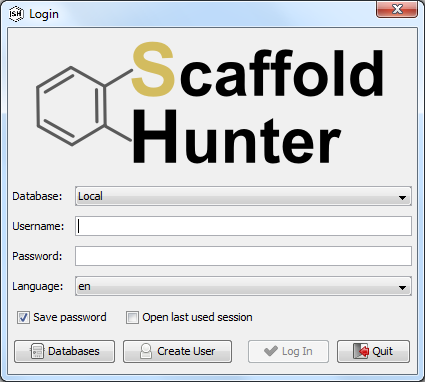
\includegraphics[scale=0.8]{images/sh_start_dialog.png}
   \caption{Start Dialog}
   \label{fig:start_dialog}
\end{figure}

The \guidialog{Start Dialog} shown in \figref{fig:start_dialog} is the first window that appears at program startup. Here you can select the database to work with and enter your username and password. If the checkbox \gui{Save password} is selected, the password will be saved in encrypted form. With the checkbox \gui{Open last used session} you can choose to automatically open the session most recently used under the given username.

    \section{Setting up a Database Connection} \label{sec:scaffoldhunter:databaseconnection}
    	\begin{figure}[ht]
   \centering
   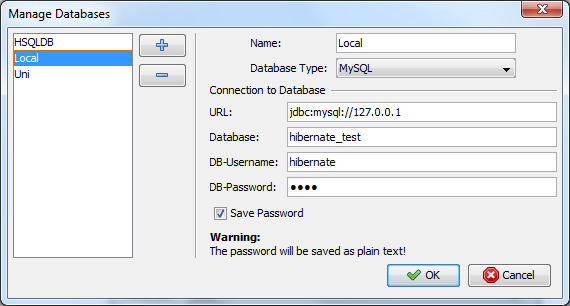
\includegraphics[scale=0.8]{images/sh_databases_dialog.png}
   \caption{Databases Dialog}
   \label{fig:databases_dialog}
\end{figure}

You can select the database to work with using the drop-down box in the \guidialog{Start Dialog}.
To add a new database to this list, click on the \gui{Databases} button.
This opens the \guidialog{Databases Dialog} shown in \figref{fig:databases_dialog}.
On the left hand side of the window, the existing database connections are shown.
With the plus and minus buttons you can create a new connection or remove an existing one.
On the right hand side the settings for the selected database are shown.

The name is only used for identification of the database connection -- you can enter any name in this field.

\gui{Database Type} is used to define the database system. At the moment \sh supports two different types of databases: \hsqldb and \mysql.

A \hsqldb database is an internal and local database.
As it is easy to configure, this database is best if you want to test \sh or to have a small private database.
If you choose a \hsqldb database, the only setting left is the database path, where you can specify a location to store the database.

\mysql is a server-based database.
It requires a \mysql server that may be running on the same machine as \sh, or on a different machine.
To configure a \mysql connection, there are a few settings to be made.
The \gui{URL} field holds the server name or IP address.
For example, ``localhost'' or ``127.0.0.1'' both would point to the local machine.
The protocol name ``jdbc:mysql://'' is not necessary and will be added automatically.
In the \gui{Database} field the database or schema name is entered.
Please note that if an existing database is entered not containing tables created
by \sh, you will be asked if you want to overwrite all existing data when connecting
to the database for the first time.
The \gui{DB Username} is used to log in to the database.
This user must be configured on the \mysql server and needs all rights to manipulate data in the database, see~\secref{sec:scaffoldhunter:requirements:database} for further information on database and user account creation.
The connection to the database also requires a password, which can be saved in the configuration file.
Please note that password is stored unencrypted.
If this password is not saved, you will be asked to enter the password each time you log in to the database.

    \section{User Management}
    	\begin{figure}[h]
   \centering
   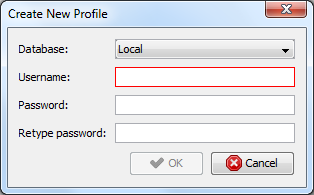
\includegraphics[scale=0.8]{images/sh_user_dialog.png}
   \caption{User Creation Dialog}
   \label{fig:user_dialog}
\end{figure}

\sh includes its own user management.
A profile is used to save personal settings and open sessions (see \subsubsecref{sec:scaffoldhunter:SessionManagement}).
To create a new user, click on the button \gui{Create User}.
Thereby the \guidialog{User Creation Dialog} shown in \figref{fig:user_dialog} is opened, where you can choose the database on which to create the user, as well as a username and password.
After clicking \gui{Ok} the program will connect to the selected database and
create a new user with the specified username. If the specified username already
exists in the database user creation will fail and an error message will be
displayed.


\chapter{Getting Started}
  \section{Session Management}
  	\label{sec:scaffoldhunter:SessionManagement}
  	In \sh, a session represents a complete working space of a user. It references a dataset consisting of molecules and a corresponding scaffold tree. The molecules of a session can be filtered to reduce the molecule count to a manageable size.

\begin{figure}[h]
   \centering
   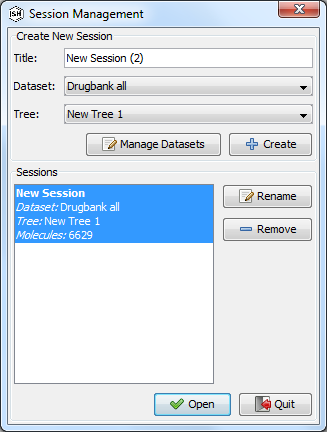
\includegraphics[scale=0.8]{images/sh_session_dialog.png}
   \caption{Session Management Dialog}
   \label{fig:session_dialog}
\end{figure}

The \guidialog{Session Management Dialog} shown in \figref{fig:session_dialog} appears after logging in, or by selecting \gui{Session $\rightarrow$ Load / Create} from the menu. If \gui{Open last used session} was selected in the \guidialog{Start Dialog}, the session management window does not appear and the last used session is opened instead. The session management consists of two areas. The upper area is used for creating new sessions. The lower area shows a list of available sessions and options for them. At the first start the session list will be empty, and a new session has to be created in order to start \sh.

To create a new session, choose a title, the dataset to create the session on, and the scaffold tree. The title can be changed later. After clicking on the \gui{Create} button, a filter dialog will appear, allowing to filter the selected dataset. The created session will then be displayed in the list of sessions in the lower area. To create a new dataset or to add a new tree to a dataset, click \gui{Manage Datasets}.

In the lower area of the session management window, the available sessions are shown with their title, dataset, tree and molecule count. Here the sessions can be renamed or removed, if they are no longer needed. To open a session, select the desired session and click the \gui{Open} button. Initially the last used session is selected in the list.

\hintbox{Important}{If you are running into database exceptions while saving a session of a larger dataset, this might be a problem with the maximum package size of \mysql. Please refer to \secref{sec:mysql_max_package_size} for further instructions about how to configure the \mysql server.}
  \section{Dataset Management} \label{sec:scaffoldhunter:datasetmanagement}
    \begin{figure}[ht]
   \centering
   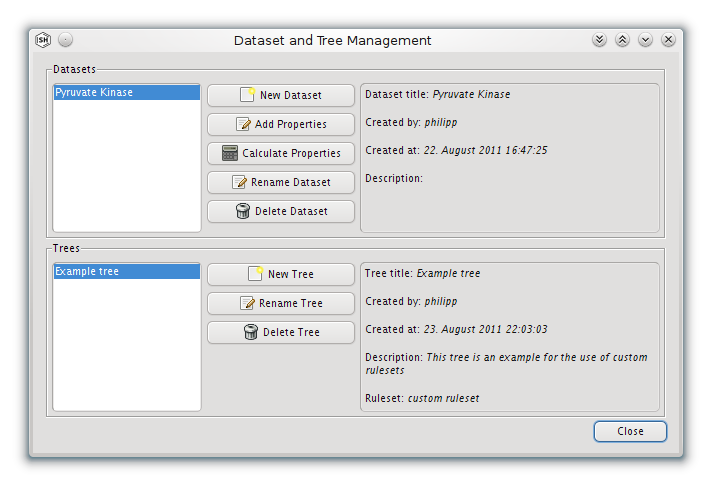
\includegraphics[width=\textwidth]{images/sh_dataset_management_dialog.png}
   \caption{Dataset Management Dialog}
   \label{fig:dataset_management}
\end{figure}

The \guidialog{Dataset Management Dialog} shown in \figref{fig:dataset_management} gives you the possibility to import, modify or delete the molecular data stored in \sh's internal database.
In \sh you can manage your projects by the use of datasets.
Each dataset consists of a set of molecules and a collection of properties for these molecules.
For each dataset you can generate an arbitrary number of scaffold trees using different generation rules.
You will later use the scaffold tree of your choice, to navigate through the molecules in the dataset.
In the following the actions you can execute on datasets and trees are explained.

\paragraph*{Actions on datasets}

\subparagraph*{New dataset}
To create a new dataset by importing chemical compound data, click on \gui{New Dataset} which opens the import wizard.
Read \secref{sec:scaffoldhunter:import} to get more information about the import process.

\subparagraph*{Add properties}
If you have an existing dataset and want to add some additional molecular properties (e.g. bioactivity information from a bio assay),
select the dataset from the list of datasets and click \gui{Add Properties}.
A wizard similar to the import wizard described in \secref{sec:scaffoldhunter:import} will appear.

\hintbox{Important}{Please note that you can only add additional properties to existing molecules.
For technical reasons it is not possible to add completely new molecules. If you try to do so, those molecules will simply be ignored.}

	
\subparagraph*{Calculate properties}
\sh gives you the opportunity to calculate additional properties (e.g. properties derived from the structure of a compound) for the molecules of a dataset.
Additionally, to enable some features like clustering molecules based on structural similarity, you may need to calculate fingerprint properties.
To calculate properties for a dataset, select the dataset from the list of datasets and click \gui{Calculate Properties}.
A dialog to create calculation tasks appears. Please read \secref{sec:scaffoldhunter:propertycalculation} to learn more about the calculation process.

\subparagraph*{Rename dataset}
If you created a dataset and would like to change its name or description, select the dataset from the list of datasets and click \gui{Rename Dataset}.
A rename dialog will appear.

\subparagraph*{Delete dataset}
If there is an existing dataset you don't need anymore, select it from the list of datasets and click \gui{Delete Dataset}.
A confirmation dialog will appear. If you confirm the deletion, the dataset and all trees in it will be deleted.

\warningbox{Warning}{\sh can be used by multiple users. If you are working on a database shared with other users, you will also destroy any work
done by other users on the dataset being deleted and the corresponding trees. First ensure nobody needs the dataset and the corresponding trees anymore.}

\paragraph*{Actions on trees}

\subparagraph*{New tree}
To create a new tree, select the dataset the tree should be generated for from the list of datasets and click \gui{New Tree}.
The tree generation dialog will appear. Read \secref{sec:scaffoldhunter:treegeneration} to learn more about how the tree generation process works.

\subparagraph*{Rename tree}
If you created a tree and would like to change its name or description, select the tree from the list of trees and click \gui{Rename Tree}.
A rename dialog will appear.

\subparagraph*{Delete tree}
If there is an existing tree you don't need anymore, select it from the list of trees on the left and click \gui{Delete Tree}.
A confirmation dialog will appear. If you confirm the deletion, the tree will be deleted.

\warningbox{Warning}{\sh can be used by multiple users. If you are working on a database shared with other users, you will also destroy any work
done by other users on the tree being deleted. First ensure nobody needs the tree anymore.}

    \subsection{Importing Data} \label{sec:scaffoldhunter:import}
      Using different \emph{import plugins}, \sh can import data from different
sources. Currently there are plugins to import data from CSV files, SDF files
and MySQL databases bundled with the program for a more detailed description of
the plugins see \subsubsecref{subsubsec:ImportPlugins}. To perform an import you
have to  create one or more import jobs, one for each data source you want to
import. These jobs will run sequentially and the data imported by those jobs
will be merged according to rules which can be selected during the import
process. In general \sh considers two structures equal if they have the same
canonical SMILES string. If a structure is present in more than one source and properties
from these sources are mapped to the same internal property the property entries
for the structure will be merged. The following \emph{merge strategies} are
available to influence which data will be found in the finished dataset:
\label{par:importing_data_merge_strategies}
\paragraph{Do not overwrite:} The first seen occurrence of the property is used and will not be overwritten by the current job.
\paragraph{Do overwrite:} The property will be overwritten by the current import job.
\paragraph{Concatenate (only for textual properties):} The property values will
be appended at the end of the existing value.
\paragraph{Minimum / maximum (only for numeric properties):} The minimum or
maximum of the available property values will be retained.

\subsubsection{Creating Import Jobs}
\begin{figure}[ht]
   \centering
   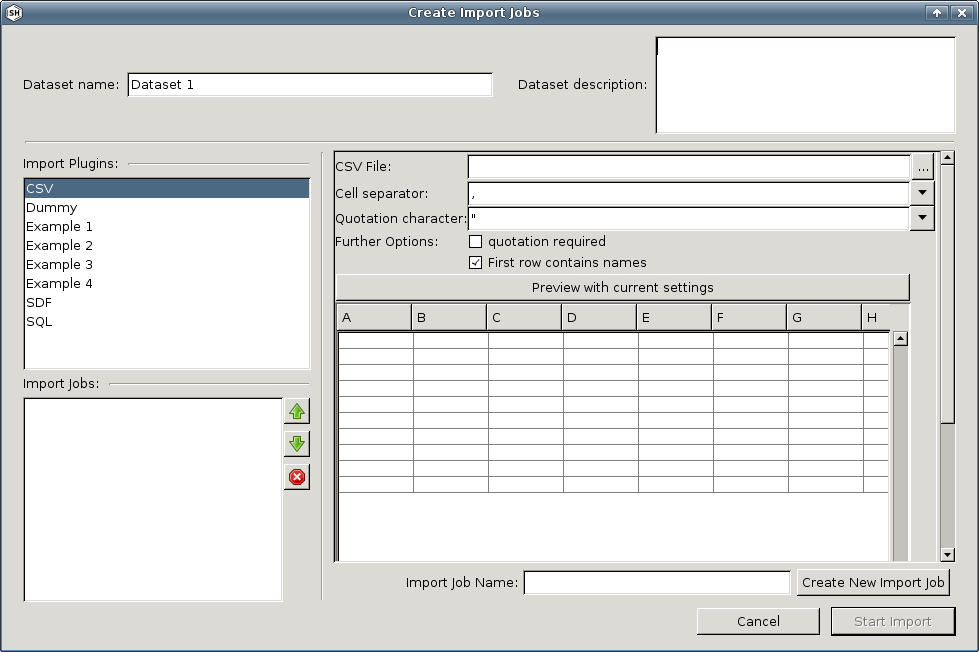
\includegraphics[width=\textwidth]{images/import/import_dialog_empty.png}
   \caption{Create Import Jobs dialog}
   \label{fig:import_dialog_empty}
\end{figure}
When you click on \gui{New Dataset} the \guidialog{Create Import Jobs} dialog
as shown in \figref{fig:import_dialog_empty} will open. In the top section
of the dialog a name and a more detailed description for the new dataset can
be entered. On the left hand side you have two lists. First the list of \gui{Import
Plugins}, where you can select a plugin appropriate for the data source you want to import.
Underneath there is the list of \gui{Import Jobs}, which contains all import
jobs created so far. The buttons beside this list can be used to delete import
jobs and to change their order. During import the jobs will be executed one after the other from top
to bottom. On the right hand side there are the settings for the currently selected plugin.
Beneath the settings you can enter an optional name for the import job. A click
on the button beside the name field will create a new import job with the
selected settings. Below this you can find a button to start the import process.

\subsubsection{Import Plugins}
\label{subsubsec:ImportPlugins}
\paragraph{CSV Import Plugin}
\begin{figure}[ht]
   \centering
   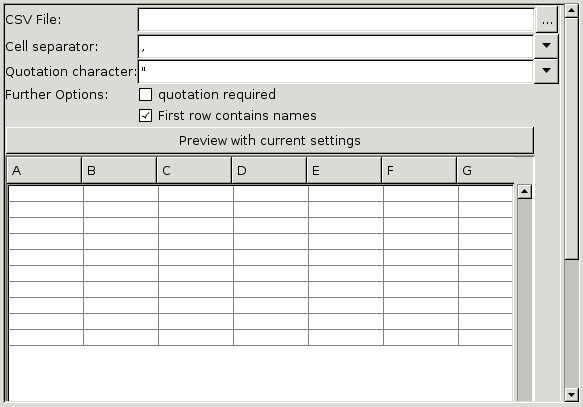
\includegraphics[width=0.5\textwidth]{images/import/csv_import_empty.png}
   \caption{CSV Import Plugin}
   \label{fig:csv_import_empty}
\end{figure} 
With the CSV plugin you can import data from comma
separated value (CSV) files. In \figref{fig:csv_import_empty} you can see
the configuration panel of the CSV plugin. You can select a CSV file, different
cell separators and quotation characters. Next to some default values you can
type in any other character. One of these options allows you to check the
\gui{quotation required} box to configure the plugin to read only quoted
content. With the \gui{First row contains names} switch you can configure the
plugin to use the first row in the CSV file for the names of the columns. If
you deselect this switch the columns will be numbered. Finally there is a
\gui{Preview with current settings} button. When you click on this button the
first 10 rows of the CSV file will be read according to your settings and
displayed in the table below. An example can be seen in
\figref{fig:csv_import_preview}.

\begin{figure}[ht]
   \centering
   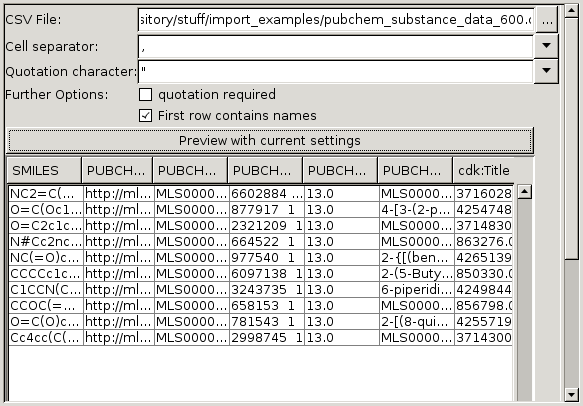
\includegraphics[width=0.5\textwidth]{images/import/csv_import_preview.png}
   \caption{CSV Import Plugin with preview}
   \label{fig:csv_import_preview}
\end{figure}

\paragraph{SQL Import Plugin}
\begin{figure}[ht]
   \centering
   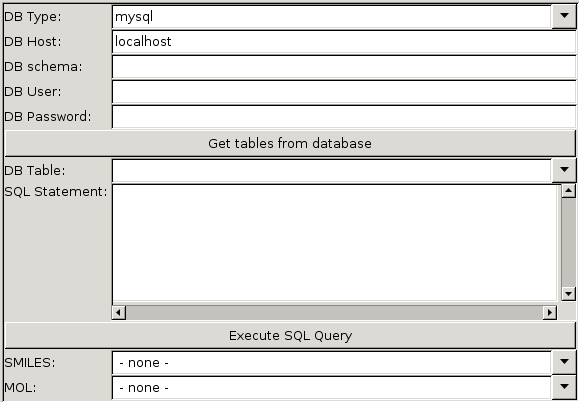
\includegraphics[width=0.5\textwidth]{images/import/sql_import_empty.png}
   \caption{SQL Import Plugin}
   \label{fig:sql_import_empty}
\end{figure}
\begin{figure}[ht]
   \centering
   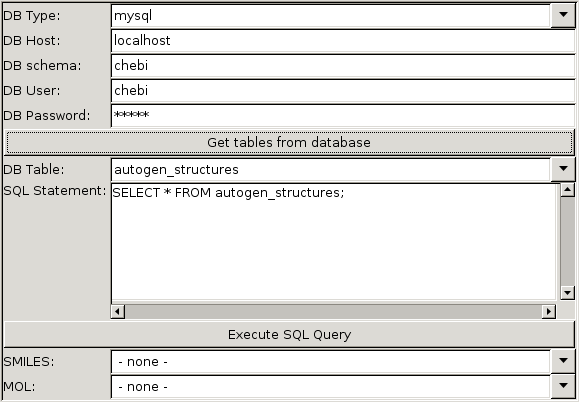
\includegraphics[width=0.5\textwidth]{images/import/sql_import_get_tables.png}
   \caption{SQL Import Plugin after \gui{Get tables from database}}
   \label{fig:sql_import_get_tables}
\end{figure}
\begin{figure}[ht]
   \centering
   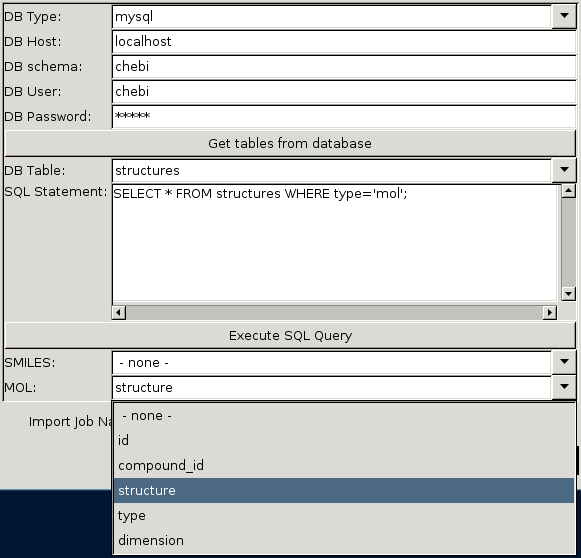
\includegraphics[width=0.5\textwidth]{images/import/sql_import_execute.png}
   \caption{SQL Import Plugin after \gui{Execute SQL Query}}
   \label{fig:sql_import_execute}
\end{figure}
The SQL import plugin allows to integrate data from SQL-based databases.
The configuration panel, as seen in \figref{fig:sql_import_empty} provides various configuration options explained in the following.
\subparagraph{DB Type}
This field allows to select the type of the SQL database you want to connect to.
Currently only \mysql is tested. Every JDBC compatible database
should be useable.  %XXX yes but they aren't
\subparagraph{DB Host}
In \gui{DB Host} you can select the database host, the server on which the source
database is running. If you need a specific port to connect to the string is: \verb+HOSTNAME:PORT+
\subparagraph{DB schema}
In the \gui{DB schema} field you can enter the database (schema) name you want to use.
\subparagraph{DB User / DB Password}
In the \gui{DB User} and \gui{DB Password} fields you can fill in your database connection credentials. Only read access is needed.
\subparagraph{Get tables from database}
Once you have entered the connection data you can click the \gui{Get tables from
database} button. The plugin will connect to the database and put all table
names found in the schema in the \gui{DB Table} list. A connection done with the ChEBI database is shown in \figref{fig:sql_import_get_tables}. 
\subparagraph{DB Table}
The \gui{DB Table} list contains the tables found after clicking on \gui{Get tables from database}. When selecting a table a  simple \verb+SELECT+ statement will be generated.
\subparagraph{SQL Statement}
In the \gui{SQL Statement} field you can type in an SQL SELECT statement that will be run on the selected database. The resulting rows from this statement will be used as source for the import.
\subparagraph{Execute SQL Query}
By clicking on \gui{Execute SQL Query} your SQL Statement will be executed and the \gui{SMILES} and \gui{MOL} lists will be filled with the resulting column names. This is shown in \figref{fig:sql_import_execute}.
\subparagraph{SMILES / MOL}
In the \gui{SMILES} and \gui{MOL} lists you can select the column names which contain structure information in SMILES and/or MOL format.

\paragraph{SDF Import Plugin}
The SDF Import plugin is very easy to use. It just has a field \gui{SDF file
name} where you enter the path to the SDF file which you want to import.

\subsubsection{Map Imported Properties Dialog}
\begin{figure}[ht]
   \centering
   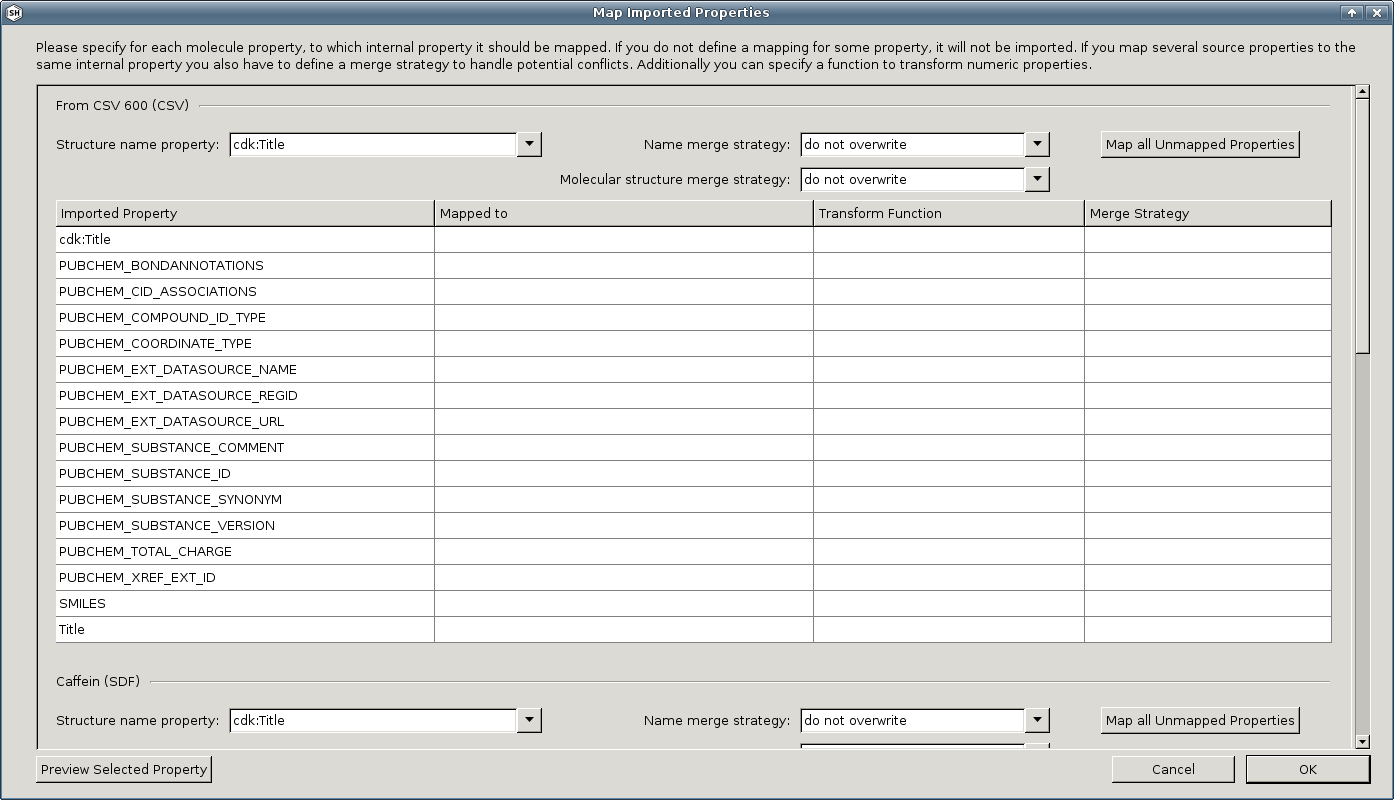
\includegraphics[width=\textwidth]{images/import/mapdialog_empty.png}
   \caption{Map Imported Properties dialog}
   \label{fig:mapdialog_empty}
\end{figure}
Once you have created at least one import job, you can start the import process
by clicking on \gui{Start Import}. A new Dialog named \gui{Map Imported
Properties} will appear. In \figref{fig:mapdialog_empty} you can see an
example of this dialog with two import jobs. For every import Job there are the
same GUI elements. At the top you have a line with the name of the following import job.
\paragraph{Structure name property}
In the \gui{Structure name property} list you select one of the properties for
the name field of the structures. The name field will be used at several places
in the program to present a name together with a structure, however it is not
used internally so there are no special requirements for this property. If the
name property is missing for some structure, the SMILES string will be used
instead.
\paragraph{Name/Molecular structure merge strategy}
In the \gui{Name merge strategy} and \gui{Molecular structure merge strategy}
you can select the merge strategies for the molecule name or 3D/2D structure
according to \parref{par:importing_data_merge_strategies}. 
\paragraph{Map all Unmapped Properties}
With the \gui{Map all Unmapped Properties} button all properties for which you
did not give  mapping information will be mapped automatically. The property
name will be the name obtained from the import plugin, the type (numeric or
text) is set also according to the plugin information as well. If multiple
sources have properties with the same name, these properties will be mapped to
the same internal property.

\hintbox{Important}{Please note that plugins typically recognize properties as
numeric only if all values of the property provided by the data source can be 
interpreted as floating point number.  As a result properties as IC$_{50}$ 
are not recognized as numeric if some values contain characters like $<$, $>$ or 
$\sim$. 
Since this may be undesirable, you may want to inspect the default mapping and
explicitly mark some properties as numeric. Values that can not be interpreted 
as floating point number will then be discarded during import.}


\paragraph{The mapping table}
In the table you have four columns. The first column (\gui{Imported Property})
shows  the property name obtained from the plugin. In the next column
(\gui{Mapped to}) you can select an existing internal property for this value,
alternatively you can choose to create a \gui{new internal property} which will
open the \gui{Create New Internal Property} Dialog (see
\subsecref{subsubsec:importing_data_create_property}) or you can choose \gui{do
not map} which will clear the table cell. In the \gui{Transform Function} column
you can input a transformation function for numerical properties, for example to
convert logarithmic to linear values. Symbols you can use are numbers, $+, -, *,
/, \verb+^+, (, ), \mathtt{log}, \mathtt{log10}, \mathtt{exp}, \mathtt{ceil}$ and
$\mathtt{floor}$. For the input value use the variable $x$. So in case you want to
convert aforementioned logarithmic values you would enter $\mathtt{exp}(x)$. In
the last column (\gui{Merge Strategy}) you can select the merge strategy for
this property. 

\paragraph{Preview Selected Property} With \gui{Preview Selected
Property} you can open a list where you can see the first 100 occurrences of the
property, which is currently selected in the table.

\subsubsection{Create New Internal Property dialog}
\label{subsubsec:importing_data_create_property}
\begin{figure}[ht]
   \centering
   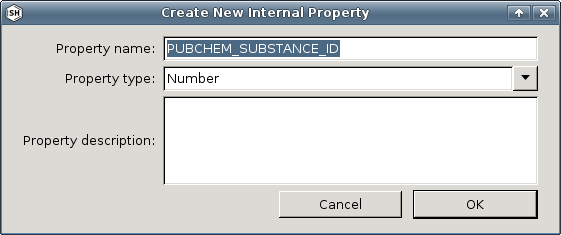
\includegraphics[width=0.5\textwidth]{images/import/create_property_empty.png}
   \caption{Create New Internal Property dialog}
   \label{fig:create_property_empty}
\end{figure}
In the \gui{Create New Internal Property} dialog, see
\figref{fig:create_property_empty} you can create new internal properties. First
you give the property a name using the \gui{Property name} field. In the
\gui{Property type} list you can select one of the property types (Number, Text, fingerprint types that can be used for clustering in the dendogram view (see \secref{sec:views:dendogram})). In \gui{Property description} you can enter a
detailed description for this property.

\subsubsection{Import into database dialog}
\begin{figure}[ht]
   \centering
   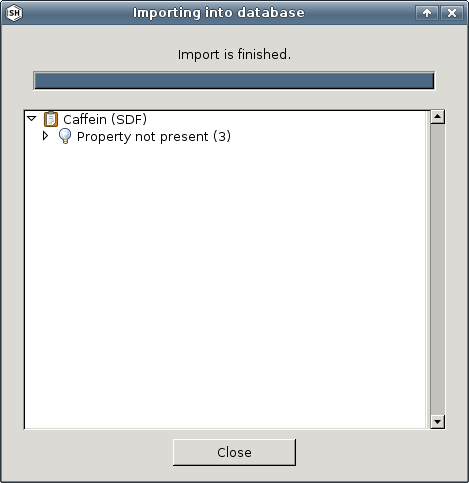
\includegraphics[width=0.5\textwidth]{images/import/import_process_finished.png}
   \caption{Importing into database dialog}
   \label{fig:import_process_finished}
\end{figure}
When you start the import in the \gui{Map Imported Properties} dialog the import
runs and the \gui{Import into database} dialog will show up. At the top you see the
current process, in the list underneath you can see some information during the
import process. When the import is finished click on \gui{Close} which concludes
creation of a new dataset.

\subsubsection{Add Properties} 
It is possible to add new properties to an existing dataset as well, by using the \gui{Add Properties} button in the \gui{Dataset and Tree Management} dialog. The process is very similar to the normal import process. However you cannot add new molecules to the dataset, due to technical reasons. Should your source contain molecules which are not contained in the current dataset, these molecules will simply be ignored during import.

Furthermore the \gui{Map Imported Properties} Dialog contains a section \gui{Merge Properties} with two fields named \gui{Source Property} and \gui{Internal Property} where you can select either to merge the datasets by molecule structure or an arbitrary property.
    \subsection{Calculation of Properties} \label{sec:scaffoldhunter:propertycalculation}
      A plugin system was integrated into \sh to support calculation of properties for the molecules of a dataset.
\sh provides a basic set of built-in plugins, and the plugin system allows users to write calculation plugins suited to their particular needs.
%If you are familiar with programming in \software{Java}, you can write your own calculation plugins.
See \chapref{chap:scaffoldhunter:writeplugins} for a detailed description how to write a plugin.\\

\begin{figure}[!htb]
   \centering
   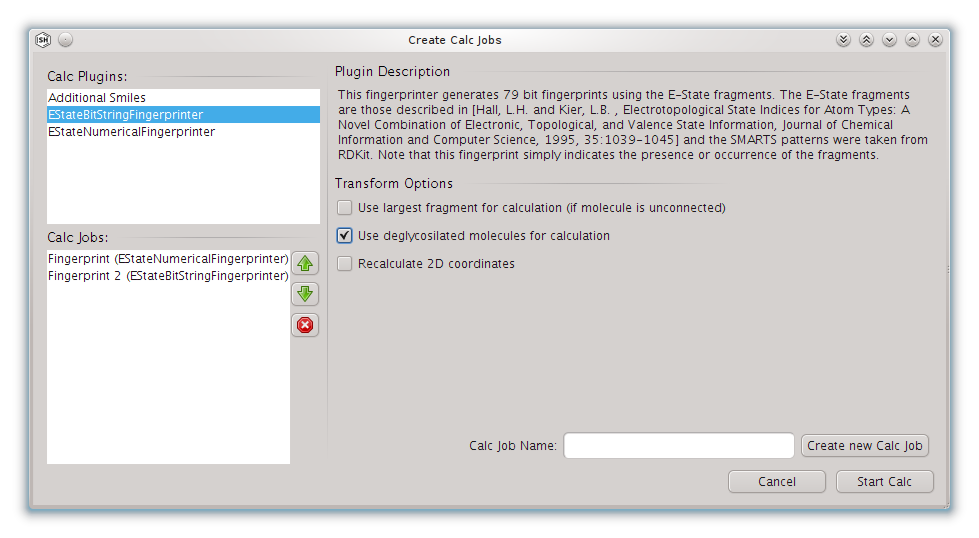
\includegraphics[width=\textwidth]{images/sh_create_calc_job_dialog.png}
   \caption{Create Calc Job Dialog}
   \label{fig:createcalcjobdialog}
\end{figure}

In the \guidialog{Create Calc Job Dialog} shown on \figref{fig:createcalcjobdialog} you can create a batch of calc jobs,
that should be executed one after each other.
Each calc job is an instance of a calc plugin, which is configured based on your needs.
Each plugin instance obtains a list of all molecules with their structural data and their existing properties,
and can use this data to calculate new properties for all (or some) molecules.
To create a batch of calc jobs, perform the following steps:

\paragraph{1. Select a calc plugin}
  In the top-left corner of the dialog you will find the list of calc plugins.
  Select one by clicking on it and proceed with the next step.

\paragraph{2. Configure the calc plugin}
  As you selected a calc plugin, the configuration panel on the right hand side of the dialog will show the plugin description
  and, depending on the plugin, a bunch of options to adjust the plugin.
  Choose the options you would like to use, and proceed with the next step.

\paragraph{3. Add the configured plugin to the list of calc jobs}
  After you have finished configuring the plugin, you can make the configured plugin instance a calc job.
  To do this, click on \gui{Create New Calc Job} in the bottom-right corner of the dialog.
  If you want to give the calc job a name, enter it in the text field labeled \gui{Calc Job Name} first. Otherwise leave the field blank.
  Now the calc job of the chosen name (or a default name) appears in the list of calc jobs in the bottom-left corner of the dialog.
  Proceed with step 1 if you want to add another calc job.

\paragraph{4. (optional) Edit the list of calc jobs}
  The list of calc jobs defines the order in which the jobs are executed.
  To change the order, select a calc job and move it up or down using the arrow buttons.
  To delete a calc job, select it and delete it by clicking on the \gui{X} button.
  If you want to change the configuration of a calc job, select it.
  The configuration panel on the right hand side of the dialog then lets you modify the job.\\

If you are ready to start the calculation, click \gui{Start Calc}.
If you want to return to the previous dialog without any changes on your dataset, click \gui{Cancel}.
After you have started the calculation, a progress window as shown in \figref{fig:calculationprogress}
will appear and inform you about the calculation status and possible issues during calculation.

\begin{figure}[!htb]
   \centering
   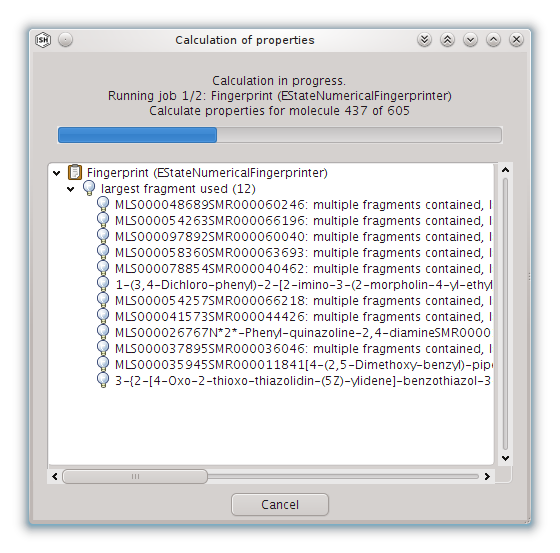
\includegraphics[scale=0.6]{images/sh_calculation_progress_dialog.png}
   \caption{Calculation Progress}
   \label{fig:calculationprogress}
\end{figure}

	
\subsubsection{Transform Options} \label{subsec:scaffoldhunter:Transform Options}
In addition to the specific options provided by each plugin, there are several plugins that provide transform options.
Transform options are used to transform the structure of all molecules, before the plugin starts the calculation.
The following transform options are available:
\paragraph{Use largest fragment}
  Sometimes multiple molecule fragments are stored (unconnected) in one single structure.
  If, for example, the plugin calculates a fingerprint which takes the molecular structure into account,
  you may want just the largest fragment of the compound to be used for the calculation.
		      
\paragraph{Use deglycosylated molecules}
  Perhaps deglycosylation (Read \subsecref{subsec:scaffoldhunter:deglycosylate} for an explanation of deglycosylation)
  has an effect on the accuracy of a calculated fingerprint.
  In this case you may want to deglycosylate before the calculation.

\paragraph{Recalculate 2D-coordinates}
  Some calc plugins (e.g. fingerprints) may depend on the 2D-coordinates of the molecules.
  If you are not sure whether all imported molecules have appropriate 2D-coordinates,
  you propably want to recalculate them for all molecules before calculating the fingerprint.


\subsubsection{Calc plugins}
Currently there are just three calc plugins available;
one plugin to calculate additional SMILES strings, and two plugins to calculate fingerprints which can be used for clustering of molecules.
Each plugin supplies its own description, so just select a plugin from the list of calc plugins as shown in \figref{fig:createcalcjobdialog} and consult the plugin description for an explanation of what the plugin does.

    \subsection{Scaffold Tree Generation} \label{sec:scaffoldhunter:treegeneration}
      \sh reduces each molecule of a dataset to its scaffold and arrange the resulting scaffolds hierarchically in a tree structure called \textit{Scaffold Tree}.
Scaffold Trees were first described by \cite{schuffenhauer_et_al2007} and allow navigation through the molecules in a meaningful manner.
In this chapter you will learn how to generate a scaffold tree.


\begin{figure}[!htb]
   \centering
   \subfloat[][Scaffold Tree Generation Dialog] {
      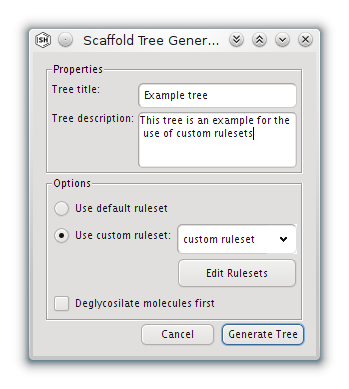
\includegraphics[width=0.45\textwidth]{images/sh_tree_generation_dialog.png}
      \label{fig:treegeneration:generationoptions}
   }
   \quad
   \subfloat[][Tree Generation Progress] {
      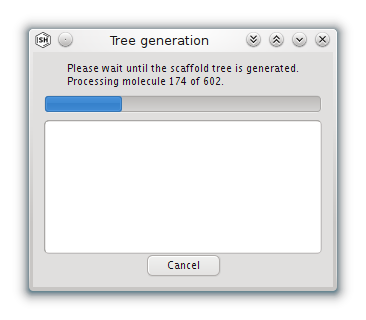
\includegraphics[width=0.45\textwidth]{images/sh_tree_generation_progress_dialog.png}
      \label{fig:treegeneration:progress}
   }
   \caption[Scaffold Tree Generation Dialog / Tree Generation Process Window]{Dialog \protect\subref{fig:treegeneration:generationoptions} allows you to configure tree generation; \protect\subref{fig:treegeneration:progress} shows the dialog indicating the process during tree generation}
   \label{fig:treegeneration}
\end{figure}


Fig. \ref{fig:treegeneration:generationoptions} shows the \guidialog{Scaffold Tree Generation Dialog}, where you have to fill in a tree title,
can fill in an explaining description of the tree and have to choose some generation options.
See \subsecref{subsec:scaffoldhunter:customrules} and \subsecref{subsec:scaffoldhunter:deglycosylate} to learn more about the options you have.
By clicking \gui{Cancel}, you will be returned to the \secref{sec:scaffoldhunter:datasetmanagement} dialog.
By clicking \gui{Generate Tree} \sh will generate and store the tree with the given options,
while showing the progress in a window shown in Fig. \ref{fig:treegeneration:progress}.
	
\subsubsection{Using Custom Rules} \label{subsec:scaffoldhunter:customrules}
The ring pruning rules define an order according to which rings are pruned from the scaffold for the generation of the scaffold tree. In 
each step of the tree generation, starting from a child scaffold, all possible parent scaffolds are generated that could be obtained by 
the removal of one peripheral ring. The hierarchical set of rules is used to select one pruning among the candidates, i.e. one ring to be 
pruned. Thereby each rule might decrease the number of candidate prunings until only a single solutions remains. In the default mode the 
rules are applied exactly as described in the Scaffold Tree publication~\cite{schuffenhauer_et_al2007}. 
To provide more flexibility with ring pruning, the custom rules option allows to define a customized subset of rules in a desired order 
selected from a wider range of implemented rules. 
For this purpose a generic framework for rules was defined. Each rule consists of two parts:

\begin{enumerate}
 \item a numerical descriptor that describes either each of the potentially pruned rings or each of the different remaining parent 
scaffolds that could be generated from the child scaffold, and 
 \item a selection criterion that defines whether the candidate prunings with the minimum or the maximum descriptor value should be 
retained (i.e. each pruning candidate except the minimum / maximum are removed from the set of remaining pruning operations) and passed 
on to the next rule until only one pruning remains.
\end{enumerate}

If multiple solutions have the minimum / maximum rule descriptor value, all of these are retained. If all pruning candidates of a 
scaffold result in the same descriptor value, all pruning candidates are passed on to the next rule.
Like with in the original ruleset, if the custom rules are not successful to identify a single pruning, a tie-break rule is evoked that 
selects the first scaffolds after lexicographically sorting the parent scaffolds according to their canonical SMILES strings.\\

To choose a set of rules for tree generation, select a ruleset from the drop-down box in the \guidialog{Scaffold Tree Generation Dialog} shown on Fig. \ref{fig:treegeneration:generationoptions}.
If no appropriate ruleset exists, you first have to click on \gui{Edit Rulesets} to open the \guidialog{Ruleset Management Dialog} and create a custom ruleset.\\

\begin{figure}[ht]
   \centering
   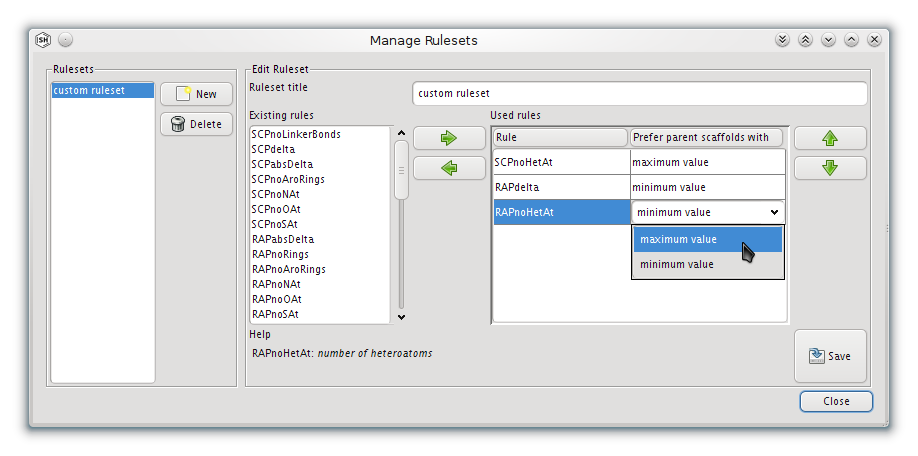
\includegraphics[width=\textwidth]{images/sh_manage_rulesets_dialog.png}
   \caption{Ruleset Management Dialog}
   \label{fig:ruleset_management}
\end{figure}

On the left side of \figref{fig:ruleset_management} you see a list of currently available rulesets.
If no ruleset is available you can create a new one by clicking \gui{New Ruleset}.

If you select a ruleset from the ruleset list, then you can edit the ruleset with the controls located on the right side of the dialog.
You have to enter a name for the ruleset and you can choose rules from the existing ruleset list on the left side of the dialog to be used in your custom ruleset.
To use a rule, select it and move it to the used rule list by clicking on the right arrow button.
You can even select and move multiple rules by using the \texttt{Shift} or \texttt{Ctrl} modifier keys during selection.\\

Each row in the used rule list represents one rule, with the descriptor name in the first column, and the selection criterion in the second column.
To change the selection criterion of a rule, select "maximum value" or "minimum value" from the corresponding drop-down box.\\

The order of the rules in the used rules list determines the order of execution of the rules.
You can change the execution order of a rule by selecting it first and then clicking on the arrow buttons to move it up or down.

If you finished editing your custom ruleset, click the \gui{Save} button to save the ruleset.\\

An adaption of the default rules within this framework would look like (for detailed explanation of the rule name see below):

\begin{verbatim}
RRPsize11p "minimum value"
SCPnoLinkerBonds "minimum value"	
SCPabsDelta "maximum value"	
SCPdelta "maximum value"
RRPsize6 "maximum value"	
RRPsize5 "maximum value"	
RRPsize3 "maximum value"	
RRPnoHetAt "minimum value"	
RRPnoNAt "minimum value"	
RRPnoOAt "minimum value"	
RRPnoSAt "minimum value"	
RRPringSize "minimum value"	
SCPnoAroRings "minimum value"	
RRPhetAtLinked "maximum value"
\end{verbatim}

\paragraph*{Implemented Rule Descriptors}
Three classes of descriptors are provided:

\begin{tabular}{lp{.5\textwidth}}
\texttt{SCP} (SCaffold Properties)       & properties of the resulting parent scaffold after pruning \\
\texttt{RAP} (Ring Assembly Properties)  & properties of the ring assembly containing the ring to be pruned \\
\texttt{RRP} (Removed Ring Properties)   & properties of the ring to be pruned \\
\end{tabular}

\paragraph*{Detailed Description of the Properties}
The names on the left are the rules that can be used in a ruleset.

\begin{longtable}{lp{0.6\textwidth}}
\textbf{Rule}			& \textbf{Description} \\
\toprule
\texttt{SCPnoLinkerBonds}	& number of acyclic linker bonds \\
\texttt{SCPdelta}		& delta value indicating nonlinear ring fusions, spiro systems bridged systems as defined in \cite{schuffenhauer_et_al2007} \\
\texttt{SCPabsDelta}		& absolute delta value indicating nonlinear ring fusions, spiro systems bridged systems as defined in \cite{schuffenhauer_et_al2007} \\
\texttt{SCPnoAroRings}		& number of aromatic rings \\
\texttt{SCPnoHetAt}		& number of heteroatoms \\
\texttt{SCPnoNAt}		& number of nitrogen atoms \\
\texttt{SCPnoOAt}		& number of oxygen atoms \\
\texttt{SCPnoSAt}		& number of sulfur atoms \\
\midrule
\texttt{RAPdelta}		& delta value \\
\texttt{RAPabsDelta}		& absolute delta value \\
\texttt{RAPnoRings}		& number of rings \\
\texttt{RAPnoAroRings}		& number of aromatic rings \\
\texttt{RAPnoHetAt}		& number of heteroatoms \\
\texttt{RAPnoNAt}		& number of nitrogen atoms \\
\texttt{RAPnoOAt}		& number of oxygen atoms \\
\texttt{RAPnoSAt}		& number of sulfur atoms \\
\midrule
\texttt{RRPringSize}		& size of removed ring \\
\texttt{RRPnoHetAt}		& number of heteroatoms \\
\texttt{RRPnoNAt}		& number of nitrogen atoms \\
\texttt{RRPnoOAt}		& number of oxygen atoms \\
\texttt{RRPnoSAt}		& number of sulfur atoms \\
\texttt{RRPhetAtLinked}		& binary descriptor (``maximum value'' = \texttt{True}, ``minimum value'' = \texttt{False}) indicating whether removed ring was linked via a linker to a heteroatom in a ring \\
\texttt{RRPsize3}		& binary descriptor: removed ring of size 3 \\
\texttt{RRPsize4}		& binary descriptor: removed ring of size 4 \\
\texttt{RRPsize5}		& binary descriptor: removed ring of size 5 \\
\texttt{RRPsize6}		& binary descriptor: removed ring of size 6 \\
\texttt{RRPsize7}		& binary descriptor: removed ring of size 7 \\
\texttt{RRPsize8}		& binary descriptor: removed ring of size 8 \\
\texttt{RRPsize9}		& binary descriptor: removed ring of size 9 \\
\texttt{RRPsize10}		& binary descriptor: removed ring of size 10 \\
\texttt{RRPsize11}		& binary descriptor: removed ring of size 11 \\
\texttt{RRPsize11p}		& binary descriptor: removed ring of size more than 11 \\
\texttt{RRPlinkerLen1}		& binary descriptor: removed ring connected via linker of length 1 \\
\texttt{RRPlinkerLen2}		& binary descriptor: removed ring connected via linker of length 2 \\
\texttt{RRPlinkerLen3}		& binary descriptor: removed ring connected via linker of length 3 \\
\texttt{RRPlinkerLen4}		& binary descriptor: removed ring connected via linker of length 4 \\
\texttt{RRPlinkerLen5}		& binary descriptor: removed ring connected via linker of length 5 \\
\texttt{RRPlinkerLen6}		& binary descriptor: removed ring connected via linker of length 6 \\
\texttt{RRPlinkerLen7}		& binary descriptor: removed ring connected via linker of length 7 \\
\texttt{RRPlinkerLen7p}		& binary descriptor: removed ring connected via linker of length more than 7 \\
\bottomrule
\caption{Rule descriptors}
\end{longtable}

\subsubsection{Deglycosylate Molecules First} \label{subsec:scaffoldhunter:deglycosylate}
This check box activates the deglycosylation of molecules that was described in \cite{Koch2005}. 
The procedure iteratively removes terminal pentose and hexose sugars based on a substructure matching before generation of the scaffold 
tree. It is especially useful when processing natural product structures, i.e. from the Dictionary of Natural Products (DNP), that 
contain molecules with multiple glycosylation patterns.

  \section{Filtering} \label{sec:scaffoldhunter:filtering}
  	\begin{figure}[ht]
   \centering
   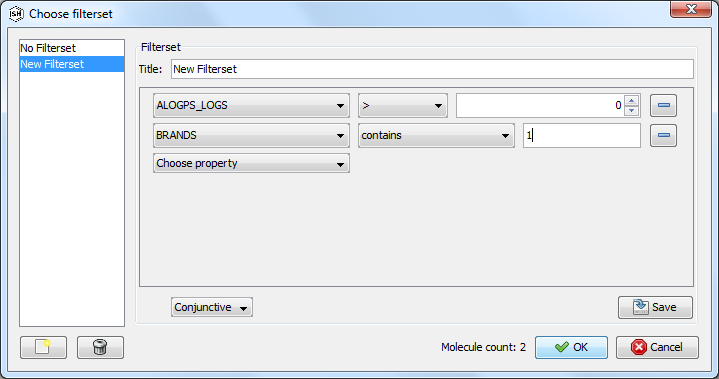
\includegraphics[width=\textwidth]{images/sh_filter_dialog.png}
   \caption{Filter Dialog}
   \label{fig:filter_dialog}
\end{figure}

The \guidialog{Filter Dialog} shown in \figref{fig:filter_dialog} is used to filter the molecules of a dataset, so that you can work with molecules relevant to your problem.
On the left hand side of the dialog a list shows the previously used filtersets.
A filterset is a set of filters.
One filter defines a constraint for one property of the molecules or scaffolds of the dataset.
A combination of filters can be used to filter the dataset by more than one property.
In the lower left corner of the window there are buttons to add a new filterset, or to delete an existing one.
After selecting one of these filtersets, or after creating a new one, the right hand side of the window shows the details of the selected filterset.
Here the title can be changed and filters can be added or modified.
To add a new filter, simply select a property from the \gui{Choose property} box.
For this property, the user can then select a constraint in the appearing drop-down box.
For numerical properties, this box holds comparison operators like ``greater'' ({$>$}) or ``equal'' ($=$).
For text properties, the user can select comparison operators like ``contains'' or ``ends with''.
Both property types can also be filtered by whether or not they are defined.
With the ``minus'' button at the end of each row, the corresponding filter can be removed.
With the \gui{conjunctive / disjunctive} box you can define the operator used to combine the filters.
With the conjunctive method, all filters have to match to allow a molecule to be added to the resulting dataset.
With the disjunctive method, only one filter needs to match.

The \gui{Save} button simply saves the changes made to the selected filterset.
To use a filterset, select it and click the \gui{Ok} button.
If the filterset was not saved before clicking \gui{Ok} and you continue without saving, the current filterset is used for filtering, but the changes are discarded afterwards.

  \section{Initial Views} \label{sec:scaffoldhunter:initial_views}
  	\begin{figure}[ht]
   \centering
   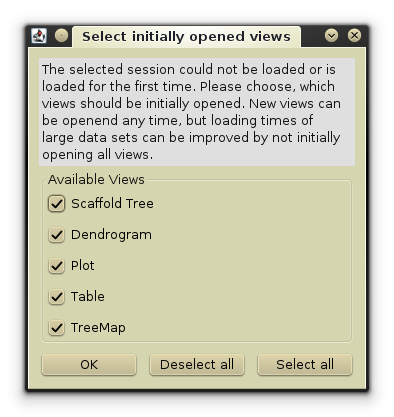
\includegraphics[width=.35\textwidth]{images/sh_initial_views.png}
   \caption{Selecting initially opened views}
   \label{fig:initial_views}
\end{figure}

When opening a session for the first time, the dialog shown in \figref{fig:initial_views} allows you to select the views that should be opened at start-up. Please note that new views can be created later at any time. However, for large datasets or in case of limited resources it is advisable to select only the required views and open additional views, e.g., for smaller subsets (see \secref{sec:scaffoldhunter:subsetmanagement}), on demand.
This reduces the loading times and memory requirements significantly.


\chapter{Main Window}
    \sh includes several \emph{views}, that allow the user to visualize and navigate through the imported chemical data in various ways.
Currently the following types of views are supported:

\paragraph{\Stview}
The \stview shows chemical structures arranged in a scaffold tree.
This is the only type of visualization that was supported by \sh version 1.x, and is still a pivotal part of the application.

\paragraph{\Dview}
The \dview shows the result of a hierarchical clustering of chemical structures, supporting various linkage methods and distance measures.

\paragraph{\Pview}
The \pview shows molecules in a two- or three-dimensional scatter plot based on the molecules' properties.

\paragraph{\Tview}
The \tview shows molecules in tabular form, including their structure, description and properties.

\paragraph{\Tmview}
The \tmview shows chemical structures arranged in a tree map. Different properties can be visualized by mapping them to the size and color of structures within the tree map.
\\

See \secref{sec:scaffoldhunter:viewmanagement} for an explanation of how to open and manage views within \sh.
The individual types of views are described in greater detail in \chapref{sec:scaffoldhunter:views}.
\\
Another concept crucial to \sh is that of subsets, as explained in \secref{sec:scaffoldhunter:subsetmanagement}.

\section{Structure of the Main Window}

The basic structure of the \sh main window stays the same regardless of the type of view that's currently in use.
However, most of the individual parts of the user interface will change when switching between different views, to accommodate the functionality of each view type.
\\
\\
The main window can roughly be divided into five parts:

\paragraph{Menu bar}
This is the main menu bar at the top of the \sh window, through which most of \sh's functionality is accessible.
Most of the menu items are available regardless of the current view.
One notable exception is the view-specific sub-menu, which changes to reflect the actions available in each given view type.

\paragraph{Tool bar}
The \tbar is located below the menu bar.
Most of the \tbar items are view-specific, and will change when switching to a different type of view.

\paragraph{View tabs}
This tab bar is the central part of the \sh window, and contains tabs for each view.
Managing views is described in \secref{sec:scaffoldhunter:viewmanagement}.

\paragraph{Side bar}
The \sbar is shown on the left hand side of the main window, and can optionally be hidden using the \gui{Show Side Bar} button in the \gui{Window} menu or in the \tbar.
It consists of several panels that can be folded or expanded independently by clicking the corresponding caption bar.
Each panel displays additional information about the data that is visible in the currently active view.

\paragraph{Subset bar}
The subset bar on the right hand side of the window shows a tree of all subsets in the current session.
Like the \sbar, this part of the user interface can be hidden, using the \gui{Show Subset Bar} button in the \gui{Window} menu or in the \tbar.
In addition to the subset tree, the subset bar also contains buttons for creating new subsets from the selection.
Subset management is explained in detail in \secref{sec:scaffoldhunter:subsetmanagement}.

  \section{Subset Management} \label{sec:scaffoldhunter:subsetmanagement}
    A central part of the \sh user interface is dedicated to the concept of \emph{subsets}.
Each subset identifies a set of molecules, all of which are part of the main dataset (hence a subset thereof).
Subsets are arranged in a tree structure, where each subset can have any number of child subsets.
Every subset is guaranteed to contain only molecules that are also in its parent subset.

At the top of the subset tree is the \emph{root subset}, which is automatically created when starting a new \sh session.
The root subset may be identical to the dataset that has been imported, but it can also be smaller in case a filter was used when creating the session.


\subsection{The Subset Tree}

The subset tree is the main part of the subset bar at the right hand side of the \sh main window.
In a newly created session, the tree contains only the root subset.
All subsets, including the root subset, can be assigned a custom name and comment.
The current subset, i.e. the subset that is shown in the currently active view, is always shown in bold.
The subset tree itself only contains the name of each subset.
Additional information about subsets can be obtained by hovering the mouse cursor above the subset name, which will pop up a tooltip window.

Most functionality regarding subsets is available using the context menu of the subset tree.
For convenience the main menu also contains the \gui{Subset} menu, which always refers to the current subset.


\subsection{Creating Subsets from the Selection}
The most straightforward way to create a new subset is by first selecting all molecules to be included in the subset, and then making a subset from the selection.
Since there is only one, global selection in \sh, which may include molecules that are not part of the current view, there are two slightly different ways to decide which molecules are to be included in the new subset.

\paragraph{Subset from the total selection}
In order to create a subset including all selected molecules, regardless of the current view, choose \gui{Selection $\rightarrow$ Make Subset} in the main menu, or use the first \gui{Make Subset} button at the bottom of the subset bar.
Since the new subset does not necessarily have any relation to any of the existing subsets, it will be added to the subset tree as a child of the root subset.

\paragraph{Subset from the selection in the current view}
To create a subset including only the selected molecules that are also in the current view, choose \gui{Selection $\rightarrow$ Make Subset from Current View}, or use the second \gui{Make Subset} button in the subset bar.
the new subset is guaranteed to include no molecules that are not part of the current view's subset, so that subset will be used as its parent.


\subsection{Deleting Subsets}

The subset of the current view can be deleted by selecting \gui{Subset $\rightarrow$ Delete} from the main menu.
In the subset tree, subsets are deleted by selecting them and choosing \gui{Delete} from the context menu.
\\
Deleting a subset always closes any open views currently associated with that subset.
\\
If the subset being deleted has any children, those will not automatically be deleted as well.
Instead, they will be re-attached to the parent of the subset being deleted.
It is not possible to delete the root subset.


\subsection{Set Operations}

The basic set operations of \emph{union}, \emph{intersection} and \emph{difference} can be used to create new subsets from existing subsets.
Since these operations require a selection of two or more subsets, they are not available in the \gui{Subset} menu, but only in the context menu of the subset tree.
\\
As in many other user interfaces, the selection of multiple subsets in the tree is possible using \texttt{Ctrl + Left click} to add or remove a single subset to/from the selection.
To select multiple adjacent subsets, \texttt{Shift + Left click} can be used.
Once all the desired subsets have been selected, open the context menu by right-clicking on one of them, and choose \gui{Make Union}, \gui{Make Intersection} or \gui{Make Difference}.
You will then be asked to enter a name for the new subset.

Since the subset tree requires each subset to be an actual subset of its parent, the set operations differ slightly in where the newly created subset will be added to the tree.
For the difference operation, the order of subsets is also relevant.

\paragraph{Union}
Generally speaking, none of the original subsets is a superset of the new subset.
As a result the new subset cannot be added below any of them in the tree.
In order to ensure that the new subset's position is both deterministic and as meaningful as possible, the parent will always be the lowest common ancestor of all the selected subsets.

\paragraph{Intersection}
All selected subsets would be a valid parent for the new subset.
For deterministic results, the subset that was clicked on when opening the context menu will be the new subset's parent.

\paragraph{Difference}
Mathematically, the difference operation is only defined for two sets.
The difference operation used here deviates from this definition by extending it to mean ``one subset, minus the union of an arbitrary number of other subsets''.
The base subset, from which the others will be subtracted, is the one that was clicked on when opening the context menu.
This is also the subset that will then become the new subset's parent.


\subsection{Reducing Subsets}
There are multiple ways to automatically create smaller subsets that are more convenient than manual selection when working with large datasets.

\paragraph{Filtering}
The same filtering that is available while creating a session can also be used on individual subsets.
Select \gui{Subset $\rightarrow$ Filter} to start filtering the subset of the current view, or choose \gui{Filter} in the context menu of any subset in the subset tree.
The \guidialog{Filter Dialog} itself works just like the one that is used during session creation, as described in \secref{sec:scaffoldhunter:filtering}.
\\
Once the filter settings have been applied, you will be asked to enter a name for the new subset, and the subset will be added to the subset tree as a child of the original subset.

\paragraph{Creating Random Subsets}
You may create a random subset of a dataset by selecting \gui{Random Subset}, either in the \gui{Subset} menu or the context menu. A dialog allows you to select the number of molecules that should be contained in the created subset.

\paragraph{Splitting by Scaffold Subtrees}
In order to create subsets based on the scaffold tree structure, you can select \gui{Split by Scaffold Subtrees}. A subset for each scaffold with a specified number of rings is created. A subset includes all molecules which belong to the scaffold or one of its descendants. Since multiple subsets are created by this function, you can specify a prefix for the newly created subsets. \sh automatically numbers the subsets consecutively and appends the number to the subset name.
  \section{Managing and Arranging Views} \label{sec:scaffoldhunter:viewmanagement}
    A newly created \sh session will contain four views, one of each type (scaffold tree, dendrogram, plot and table), with each view showing the root subset.
This setup is meant to serve only as a starting point.
The number of simultaneous views is only limited by the system's available memory, and each view can be associated with a different subset and different settings.


\subsection{Opening and Closing Views}

There are several ways of creating a new view.
The \gui{Window $\rightarrow$ Add View} submenu can be used to create a new view of a given type, showing the root subset.
A more flexible way of opening new views is using either the \gui{Subset} menu or the subset tree's context menu:

\begin{description}
    \item[Show in Current View] (only in subset tree context menu) \hfill \\
    Replaces the subset shown in the currently active view, while otherwise retaining the view's settings.
    \item[Show in New View] \hfill \\
    Creates a new tab in the current window, showing the selected subset in the chosen type of view.
    \item[Show in New Window] \hfill \\
    Creates a new window and adds a new tab to it, showing the selected subset in the chosen type of view.
\end{description}

\noindent Note that the \gui{Subset} menu always refers to the current view's subset, while the context menu refers to the subset being clicked on.

Usually the fastest way to close a view is by using the 'X' button in the view's tab, but there are also menu items (\gui{Window $\rightarrow$ Close View}) and a keyboard shortcut (\gui{Ctrl+W}) available.


\subsection{Split Windows}

It is possible to simultaneously show two views in the same window, either side by side or one above the other.
To split the window, use \gui{Window $\rightarrow$ Split Horizontally} and \gui{Window $\rightarrow$ Split Vertically}.
This will create a new, initially empty tab bar, that can then be filled by moving views to it (see \subsecref{sec:scaffoldhunter:viewmanagement:moving}).
The same menu items can also be used to change the orientation of an existing split.

To get back to a window with no split, use \gui{Window $\rightarrow$ Single Tab Bar}.
This will join all views from both sides of the split in a single tab bar.


\subsection{Multiple Main Windows}

Sometimes it can be convenient to open views in separate windows, for example to place them on different monitors, or to avoid a tab bar getting too crowded.
\sh supports this by allowing multiple main windows within the same instance of the application.
Windows can be opened using \gui{Window $\rightarrow$ Open New Window}, and closed using \gui{Window $\rightarrow$ Close Window}.
Note that while each window can have its own views and layout, all windows still work on the same dataset and subset tree.
Thus, opening multiple main windows is not the same as opening multiple instances of \sh.


\subsection{Moving Views} \label{sec:scaffoldhunter:viewmanagement:moving}

Within a single tab bar, views can easily be moved by simply dragging their tab to a new position.\\
It's currently not possible to move views to a different tab bar (in case of split views) or to a different window via drag \& drop.
To move windows from one window or tab bar to another, use \gui{Window $\rightarrow$ Move View to Window} and \gui{Window $\rightarrow$ Move View to Tab Bar}.


\subsection{Renaming Views} \label{sec:scaffoldhunter:viewmanagement:renaming}

Views are initially named after their type.
For example, the tab of a newly created \stview will be called ``Scaffold Tree''.
Views can be renamed to give them a more descriptive label.
To do so, select \gui{Window $\rightarrow$ Rename View} in the main menu, or \gui{Rename} in the tab's context menu.

  \section{Interaction between Views}
  	\subsection{Selection}
\label{sec:linking:selection}

In order to create subsets containing molecules of interest it is possible to select several molecules in the views, which are then highlighted in red in all views.

Single molecules or the molecules belonging to a scaffold can be selected or deselected by left clicking a molecule or a scaffold or in some views by dragging a selection box around them or by using the scaffold's context menu.
Another possibility to change the selection is the subset menu. If the menu has been opened via the main menu, it offers options to add the current subset of the active view to the selection, to remove it, or to replace the selection. The same applies to the subset which has been used to open the context menu in the subset bar.

The user can also select all molecules of the dataset, clear the selection, invert the current selection or confine the current selection to the molecules that are visible in the active view by using the selection menu in the main menu.

The total number of molecules selected and the number of molecules selected that are visible in the active view are displayed at the bottom of the subset bar. Both have an associated \gui{Make Subset} button that can be used to create a new subset from the respective set.

\paragraph{Selection colors}

\tableref{tab:selectioncolors} shows the possible colors of molecules and scaffold, depending on their selection state:
\\

\begin{table}[ht] 
  \centering
 \begin{tabular}{rl}
\textbf{Display color} &
  \textbf{Selection state} \\ \toprule
\textcolor{black}{black} &
  Unselected molecule or scaffold \\
\textcolor{red}{red} &
  Selected molecule \\
\textcolor{red}{red} &
  Completely selected scaffold (all molecules belonging to the scaffold are selected) \\
\textcolor{orange}{orange} &
  Partially selected scaffold (some molecules belonging to the scaffold are selected) \\
\textcolor{gray}{gray} &
  Virtual scaffold (scaffold with no child molecules; cannot be selected) \\ \bottomrule
\end{tabular}
  \caption{Selection colors}
  \label{tab:selectioncolors}
\end{table}



\subsection{Flags}
\label{sec:linking:flags}

Besides the selection, there is another kind of marking that is shared by all views: flags. Flags are intended as a fast way of marking molecules and scaffolds, for example as \textit{already seen} or \textit{investigate later}, and are available in a \textcolor{green}{public} and in a \textcolor{blue}{private} variant. Public flags are visible to everyone working on the dataset, while private flags are only visible to the user who created them.

The user can mark molecules and scaffolds with flags by using the context menu or the main menu entry \gui{Selection}.
If the context menu is used, the private and public flags of the molecule or scaffold under the cursor can be toggled.
The selection menu allows the user to add or remove a public or private flag for all molecules of the current selection.

  \section{Tooltip Window and Comments}
    \begin{figure}[!htb]
   \centering
   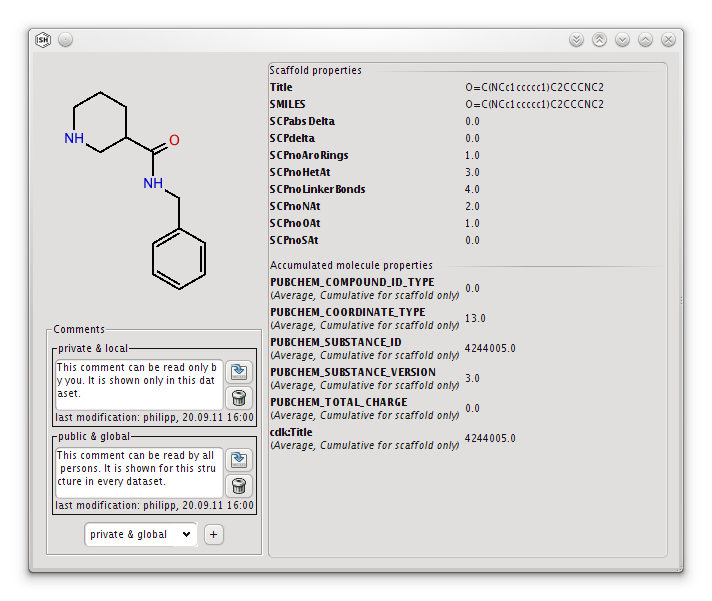
\includegraphics[width=0.5\textwidth]{images/sh_tooltip_dialog.png}
   \caption{Tooltip}
   \label{fig:tooltip}
\end{figure}
An interactive tooltip window (see \figref{fig:tooltip}) is available for the \stview and the \dview when you move your mouse over a molecule or scaffold. It combines the following components in one window. 
\begin{itemize}
 \item a large \textbf{image} of the structure
 \item configurable information on the \textbf{properties}
 \item a component to view, add, delete or modify \textbf{comments}
\end{itemize}
The window behaves different from a normal tooltip in some circumstances. Like a normal tooltip it disappears as soon as the mouse leaves molecule, scaffold or tooltip window. But if you click inside the window the window will stick and stay until the focus of the window is lost. This enables you to move around the mouse freely and (more important) lets you edit the comments more safely.

\subsection{Configuring the Tooltip}
You can find some general options at \texttt{Session $\rightarrow$ Preferences $\rightarrow$ General Configuration} in the menu bar. 
\begin{itemize}
 \item \textbf{enable/disable} tooltip
 \item the \textbf{size} of the image shown in the tooltip
 \item whether it shows \textbf{undefined properties} or not
 \item the \textbf{delay} after which the tooltip is shown
\end{itemize}

\subsection{Configuring the Properties}

\begin{figure}[!htb]
   \centering
   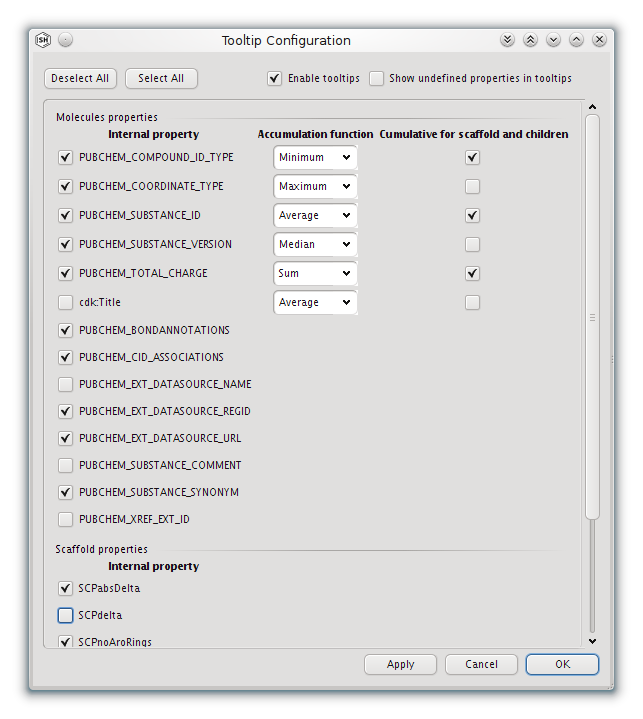
\includegraphics[width=0.5\textwidth]{images/sh_tooltip_configuration_dialog.png}
   \caption{Tooltip Configuration}
   \label{fig:tooltip_configuration}
\end{figure}

You can find a dialog to configure the properties at \texttt{Session $\rightarrow$ Tooltip Configuration} in the menu bar. As you can see in \figref{fig:tooltip_configuration} you have a check box in front of every property to enable or disable the property in the tooltip. As the tooltip can be shown for molecules and scaffolds there are two types of properties. If the tooltip is displayed over a molecule only the molecule properties will be shown. 

The properties for scaffolds are somewhat more complex. You can derive accumulated properties for scaffolds from the molecule properties that belong to the displayed scaffold. Therefore you can choose an accumulation function for each numerical molecule property. For example you can display the average, minimum or maximum of the molecule property when using the tooltip with scaffolds. 
If you enable the checkbox \texttt{Cumulative for scaffold and children} this accumulation function is applied to the molecules of the scaffold and all molecules that belong to any child scaffold.

\subsection{Comments}
You can add, modify and delete comments for a molecule or scaffold directly in the tooltip. You can find the controls in the bottom left corner of the tooltip (see \figref{fig:tooltip}). 

\paragraph{Private, public, local and global comments}
Comments can be private or public and local or global. Therefore you have 4 different types of comments (private \& local, private \& global, public \& local, public \& global). If a comment is private it is only accessible by the user who created it, while a public comment can be seen by any other user working on the same database. If a comment is local it is limited to the current tree. If you choose global instead it will be visible for all datasets and all trees on the current database for molecules or scaffolds with the same structure.

\paragraph{Add, modify or delete a comment}
To add a new comment select the type in the drop-down box and click the plus button. Note that only one comment of each type can exists for each molecule or scaffold. Therefore not all or no types may be available in the drop-down box. After adding a new comment a text field with a save button, delete button and some information about the modification will appear. You can now modify the (empty or previously existent) comments by editing the text in the text field and pressing the save button afterwards. The save button will be only accessible if you already modified the text. Otherwise it will be greyed out. To delete a comment simply press the delete button. The text field with the according controls will disappear.

  \section{Settings}
    The \sh settings are divided into two types. There are global preferences and settings for a specific view. All settings are stored in the database. Therefore your settings travel with your profile.

\begin{figure}[!htb]
   \centering
   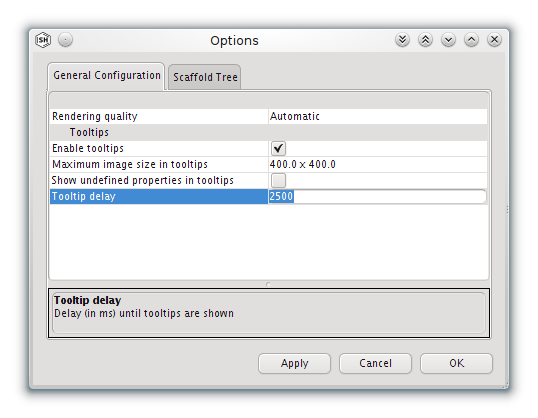
\includegraphics[width=0.5\textwidth]{images/sh_preferences_dialog_generalconfiguration.png}
   \caption{Preferences Dialog}
   \label{fig:generalconfiguration}
\end{figure}
\paragraph{Preferences}
The global preferences are accessible via \texttt{Session $\rightarrow$ Preferences} in the menu bar. The Dialog \figref{fig:generalconfiguration} has a \texttt{General Configuration} tab with settings that will apply to all views and the main window. The options are self explaining. If you select an option by clicking on it you get a more detailed description in the label below. 

There are also tabs for types of views. For example you can find general options for the \stview. These settings will apply to all views of one type that are open (e.g. all \stviews). Currently only the \stview uses this global settings, but in future there may be also other views available here. 

\begin{figure}[!htb]
   \centering
   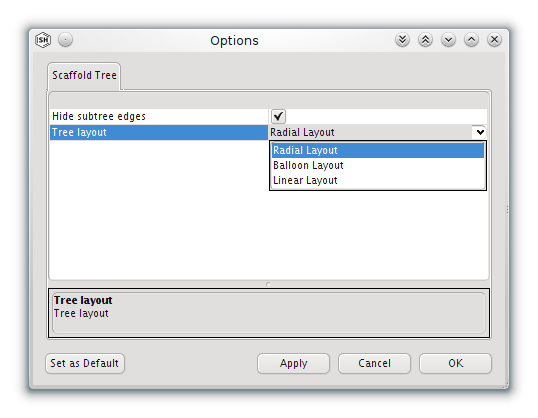
\includegraphics[width=0.5\textwidth]{images/sh_configure_view_dialog_scaffoldtree.png}
   \caption{Configure View Dialog}
   \label{fig:configure_view}
\end{figure}
\paragraph{Configure View}
The preferences for one specific view are accessible over \texttt{Session $\rightarrow$ Configure View}. The dialog \figref{fig:configure_view} has the same layout as the global preferences. It shows one tab for each open view. If you have two open \stviews you will find two tabs here. The name of the tabs matches the name of the view tabs in the main window. Renaming the views can thereby significantly improve the assignment between preferences tabs and the corresponding view (see \secref{sec:scaffoldhunter:viewmanagement:renaming}). Some options may also be available directly over the menu bar or \tbar (for further details see \secref{sec:scaffoldhunter:views}).

\chapter{Views} \label{sec:scaffoldhunter:views}
	This chapter will give you a deeper understanding of each available view. If you want to know how to handle, manage and arrange views in general terms you may want to read \secref{sec:scaffoldhunter:viewmanagement} instead. 
  \section{Scaffold Tree}
    The \stview visualizes a \stree, which was generated as described in 
\subsecref{sec:scaffoldhunter:treegeneration}. 

\subsection{Navigation}
A new \stview will show an overview of the whole graph. You may zoom in to get
more detailed information on a part of the graph. Depending on the scale,
scaffolds will be represented simplified by a rectangle or by their structural
formula. There are several ways to zoom in/out: You may use the mouse wheel to
magnify/demagnify the view on the area of the mouse pointer or by using the
buttons in the \tbar or \gui{Tree} menu. You may also select the area of
interest by a rectangle on the GraphMap, see
\subsecref{sec:treeview:graphmap}. The other navigation mechanism is
panning: By keeping the left mouse button pressed on an empty area in the graph
pane and moving the mouse the viewpoint is panned. You may also use the
scrollbars for panning.

Usually not all scaffolds are shown when a new \stview is opened. Subtrees
beginning at a scaffold can be shown or hidden respectively by clicking on the
+/-- symbol at the lower left corner of the scaffold. In addition, the context menu
(\subsecref{sec:treeview:contextmenu}) contains options to open complete
subtrees or to open all children on the next hierarchy level. Inverse operations
exist to hide scaffolds you are not interested in. The command to expand the
whole tree or to reset it to the default hierarchy level can be invoked via the
\tbar or  \gui{Tree} menu (\subsecref{sec:treeview:menutoolbar}).

A scaffold will be shown in different colors based on the global selection as
described in \subsecref{sec:linking:selection}. A left-click on an unselected or
partially selected scaffold will add all molecules associated with the scaffold
to the selection, a left-click on a fully selected scaffold will deselect all
associated molecules.

You may also navigate using keyboard shortcuts, listed in
\appref{chap:scaffoldhunter:shortcuts}. There is a cursor set on one scaffold
marked by a blue rectangle. The cursor can be  moved using the arrow keys. The
camera automatically retains focus on the cursor.


\subsubsection{GraphMap} \label{sec:treeview:graphmap}
The GraphMap is found in the \sbar on the left hand side and provides an
overview on the whole graph. The current viewport of the graph pane is marked by
a transparent red rectangle. Dragging this rectangle with the mouse will change
the viewport of the graph pane accordingly. Click the left mouse button at an
area that is not currently visible to center the viewport on the selected point.
You can define a new viewport by marking a rectangle on the graph map: Click the
left mouse button on an empty area and keep it pressed while moving the mouse.
When releasing the mouse button the view will be panned and zoomed to completely
contain the selected area. Using your mouse wheel on the GraphMap will magnify
or demagnify the graph pane at the specified point.

\subsubsection{Magnifying Glass}
The Magnifying Glass in the \sbar below the GraphMap is opened by a mouse click on its title bar. It shows the area below the mouse 
pointer magnified. You may move the mouse pointer over the graph pane and navigate in the graph as usual while the Magnifying Glass is 
active.



\subsection{Context Menu} \label{sec:treeview:contextmenu}
\begin{figure}[!htb]
   \centering
   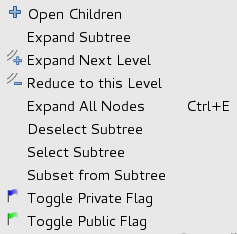
\includegraphics[width=0.3\textwidth]{images/stree/contextmenu.png}
   \caption[\Stview contex menu]{The context menu invoked by a right-click on a scaffold.}
   \label{fig:scaffoldhunter:contextmenu}
\end{figure}
Click the right mouse button on a scaffold to access the context menu. The menu mainly contains options that are directly related to the 
scaffold: You can open/close the children of the scaffold, open the whole subtree rooted at the scaffold or open all children on the next 
hierarchy level by the option \gui{Expand next level}. In addition you can
choose to expand the whole tree, by clicking on \gui{Expand all Nodes}. You can
hide the hierarchy levels under the scaffold by choosing \gui{Reduce to this
level}.

The commands \gui{Select Subtree} and \gui{Deselect Subtree} add or remove all
molecules from the selection, which are associated with scaffolds located in the
subtree that is rooted at the current scaffold. The command \gui{Subset from
Subtree} will create a new subset which contains these molecules.

There are two additional entries to set or remove public and private flags, see
\subsecref{sec:linking:flags}.

\subsection{Tree Menu \& Tool Bar} \label{sec:treeview:menutoolbar}
\begin{figure}[!htb]
   \centering
   
\includegraphics[width=0.9\textwidth]{images/stree/toolbar.png}
   \caption[\Stview \tbar]{
      Meaning of the icons (from left to right): Zoom In, Zoom Out, Fit Graph,
      Fit Selection, Expand all Nodes, Number of Rings to Default Level,
      Increase/Decrease Radius, Lock Radii while Zooming, Scale cusor node
      up/down, Normalize cursor node, Scale Selected Scaffolds up/down,
      Normalize Selected Scaffolds, Normalize all Scaffolds, Configure Property
      Mappings, Show Scaffold Molecules, Export Image
   }
   \label{fig:treeview:toolbar}
\end{figure}

The \gui{Tree} menu provides access to many different functions related to the
\stview. The \tbar shown in \shortfigref{fig:treeview:toolbar} allows quick
access to most of these functions. When you hover the cursor over an item of the
menu or \tbar a tooltip with a description will appear. It follows a list of
the menu items, each with a short description.

\begin{description}
 \item [Layout] Can be used to choose one of the three available layout algorithms. The graph in the current tab will be laid out accordingly. 
See \subsecref{sec:treeview:layout} for a brief description of the layouts.
 \item [Show Scaffold Molecules] Toggles the molecule view for each node in the
 scaffold tree, which displays the molecules associated with a scaffold.
 \item [Configure Property Mappings] Allows to map different imported
 properties to several visual features of the nodes in the \stree{}. See
 \subsecref{sec:treeview:propertymappings} for details.
 \item [Zoom In/Out] Changes the zoom level of the graph pane.
 \item [Fit Graph] Changes the zoom level and pans the graph pane to show the
 whole graph.
 \item [Fit Selection] Changes the zoom level to show all selected and partially
 selected scaffolds.
 \item [Expand all Nodes] Expands the whole Graph.
 \item [Number of Rings to Default Level] Resets the graph, such that only the
 hierarchy levels which are shown by default are displayed.
 \item [Increase/Decrease Radius] Allows adjustment of the distance between two
 adjacent rings in the radial layout.
 \item [Lock Radii While Zooming] Disables/enables the automatic adjustment of the distance
 between two adjacent rings in the radial layout.
 \item [Node Scale] Resizes the scaffolds of the graph. There are buttons for
 scaling up/down all currently selected scaffolds or just the scaffold the
 cursor is on. In addition \gui{Normalize} buttons are provided to reset
 scaffolds to their original size.
 \item [Export Image] Allows exporting the current viewport or the whole graph
 as an image. 
\end{description}

\subsection{Layout} \label{sec:treeview:layout}
\begin{figure}[!htb]
   \centering
   \subfloat[][] {
      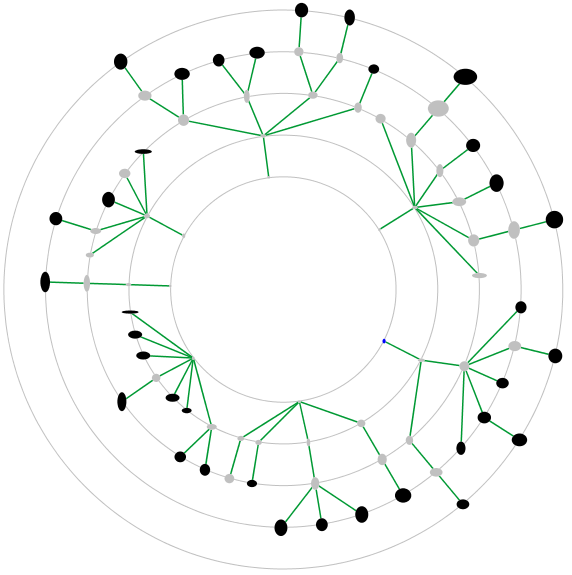
\includegraphics[scale=0.3]{images/stree/sh_layout_radial.png}
      \label{fig:treeview:layout:radial}
   }
   \quad
   \subfloat[][] {
      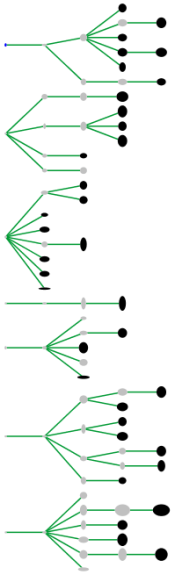
\includegraphics[scale=0.3]{images/stree/sh_layout_linear.png}
      \label{fig:treeview:layout:linear}
   }
   \quad
   \subfloat[][] {
      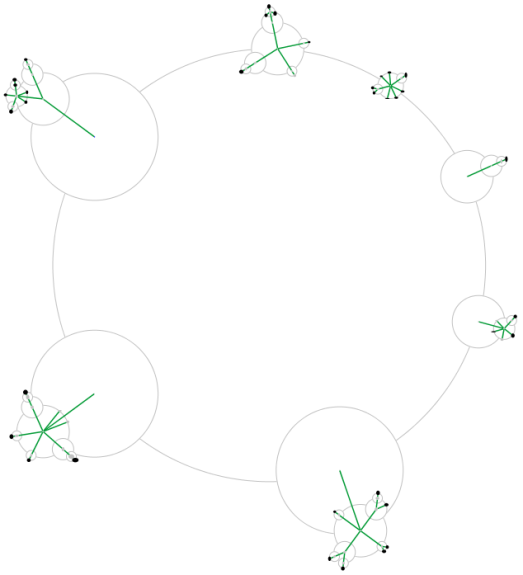
\includegraphics[scale=0.3]{images/stree/sh_layout_balloon.png}
      \label{fig:treeview:layout:balloon}
   }
   \caption[\Stview layouts]{
      Different layouts of the same graph: \subref{fig:treeview:layout:radial} Radial Layout, \subref{fig:treeview:layout:linear} Linear Layout, \subref{fig:treeview:layout:balloon} Balloon Layout
   }
   \label{fig:treeview:layout}
\end{figure}
\sh offers three different layouts, which can be selected by using the
\gui{Layout} option in the \gui{Tree} menu \subsecref{sec:treeview:menutoolbar}.
The different layouts are shown in \shortfigref{fig:treeview:layout}. The Radial Layout
(\shortfigref{fig:treeview:layout:radial}) is the default layout method. 
With this layout the scaffolds are located according to their depth on circles
with a common center. The Linear Layout (\shortfigref{fig:treeview:layout:linear}) orders the
scaffolds from left to right. Both layouts emphasize the depth of scaffolds.
With the Balloon Layout (\shortfigref{fig:treeview:layout:balloon}) each scaffold is the
center of a circle on which its children are distributed. This 
layout separates subtrees more clearly from each other.

For the Radial Layout the distance between the circles may be customized. By default the
distance is automatically adjusted depending on the zoom. The \gui{Lock Radii
While Zooming} button disables this mechanism and allows the user to set the
distance using the buttons \gui{Increase Radius}/\gui{Decrease Radius}.

\subsection{Sorting}
Initially the ordering of scaffolds in the tree is chosen in a deterministic
way but without any meaning. Alternatively scaffolds can be sorted according to
some property value using the \gui{Sort} \sbar panel
show in \shortfigref{fig:treeview:sortpanel}.

The same panel can be used to define the ordering of the molecules which are
shown when the option \gui{Show Scaffold Molecules} is toggled. To do so select
the property by which these molecules should be sorted in the uppermost box.

\begin{figure}[!htb]
   \centering
   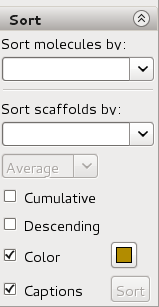
\includegraphics[scale=0.5]{images/stree/sidebar_sort.png}
   \caption{The Sidebar sort panel}
   \label{fig:treeview:sortpanel}
\end{figure}
The property used for sorting can be chosen using the box below \gui{Sort
Scaffolds by}. An accumulation method to determine how scaffold
properties will be derived from the properties of associated molecules can be selected in the
box below. The checkboxes underneath can be used to add a colored background to
the graph, where each segment which has the same value of the selected property
is colored in the same shade of the selected color. A label showing this value
can be displayed in each segment.

After clicking on \gui{Sort} the scaffolds on the first layer will be reordered
according to their property values. Sorting by property values is applied only
to the scaffolds on the first layer. You can however create a subset out of a
subtree and sort the \stree displaying the subset. 

\subsection{Property Mappings}
\label{sec:treeview:propertymappings}
Properties associated with the scaffolds can be mapped to different \emph{visual
properties} of the Scaffold Tree. Scaffold properties are either directly
associated with a scaffold, such as \emph{Number of Oxygen Atoms} or can be
derived from the properties of the structures  which are associated with a
scaffold.

The following \emph{visual properties} are available for mapping:

\paragraph{Node Background Color} This changes the background color of the
scaffold nodes in the scaffold tree. Either two colors can be selected and the
value range of the property is mapped to the gradient between those two colors
or value intervals can be specified and a color can be assigned to each
interval.

\paragraph{Edge Thickness} This maps the absolute difference between the values
associated with two adjacent scaffolds onto their connecting edge. The maximum
and minimum displayed thickness are predefined and cannot be adjusted. A
gradient mapping maps the greatest difference to the maximum thickness and the
smallest difference to the minimum thickness, intermediate differences are linearly
mapped to intermediate thickness values. Alternatively intervals of differences
can be defined, which will then be mapped to different thickness values.

\paragraph{Edge Color} Similarly to the way values can be mapped to the
background color of a node they can also be mapped to the adjacent edges. On the
edge a gradient between the colors will be displayed, which is determined by the
adjacent scaffolds.

\paragraph{Label} The value associated with a scaffold can be displayed by a
label below the node in the scaffold tree. 

\begin{figure}[h]
\centering
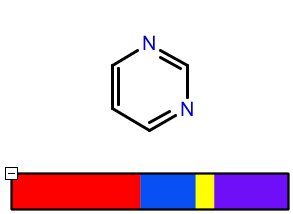
\includegraphics[scale=0.5]{images/stree/infobar.png}
\caption{An example of an Info Bar.}
\label{fig:treeview:infobar}
\end{figure}

\paragraph{Info Bar} This visualizes distributions of a property for the
molecules associated with a scaffold. Intervals can be specified and a
color is associated with each interval. The distribution of these intervals can then
be visualized as shown in \shortfigref{fig:treeview:infobar}. Textual properties
with ten different values or less can also be mapped to colors to display such a
distribution.

\begin{figure}[p]
\centering
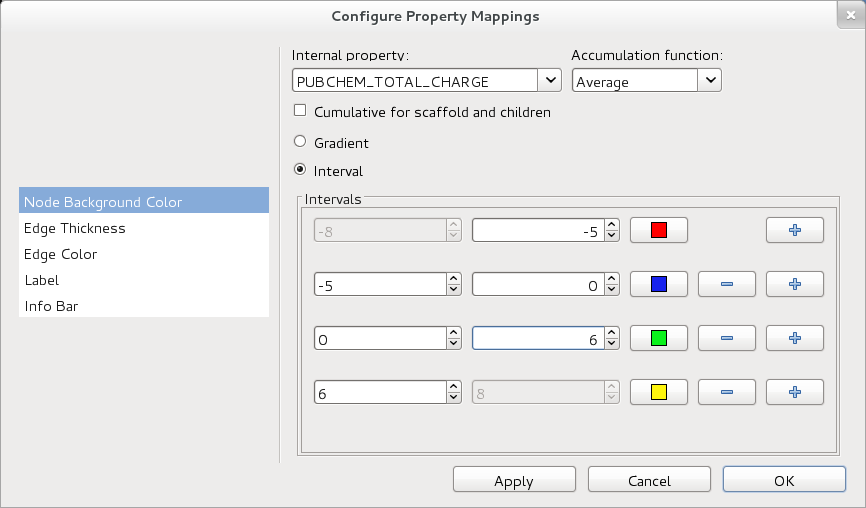
\includegraphics[scale=0.5]{images/stree/mappingdialog.png}
\caption{The property mapping dialog showing an interval mapping to the Node
Background Color.}
\label{fig:treeview:propmapdialog}
\end{figure}

The dialog to configure these mappings is shown in
\shortfigref{fig:treeview:propmapdialog}. On the left the visual property can be
selected, on the right settings for the selected visual property can be
configured. These settings may vary depending on the visual property. In general
the scaffold property to be mapped can be selected using the box at the top, in
case of \emph{derived properties} a second box will be displayed to select the
accumulation function. If the box \gui{Cumulative for scaffolds and children} below
is selected the accumulation function will not only be applied to values of
the structures associated with the scaffold, but also include the
values of all structures, which belong to scaffolds located in the subtree below
the scaffold.

\subsection{Exporting Images}
\label{sec:treeview:imageexport}

\begin{figure}[p]
\centering
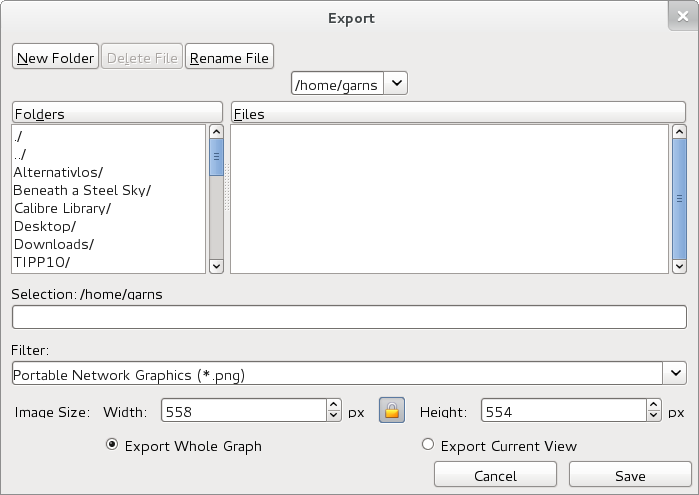
\includegraphics[scale=0.5]{images/stree/export.png}
\caption{The export dialog.}
\label{fig:treeview:export}
\end{figure}
Clicking the \gui{Export Image} button in the \tbar or the \gui{Tree} menu
will open the export dialog shown in \shortfigref{fig:treeview:export}, which
allows you to save the current graph as an image. You can either  export the
current view on the graph, which will save only the part of the graph
which is currently visible in the graph pane, or the whole graph. There are
three file formats available (SVG, PNG and TIFF) and options to control the
image size. By default the aspect ratio of the exported image is fixed, this can
be changed by clicking on the lock.

Since SVG is a file format for vector graphics the exported image can
be scaled without quality loss. Consequently the specified image size will not
have much effect on the quality or file size for SVGs but is very important for
raster formats such as PNG and TIFF. Even if the current view shows rectangles
for scaffolds the exported image will always show their structural formulas. 

\newpage

  \section{Table} \label{sec:scaffoldhunter:table}
    An overview of the aggregated molecule information can be seen in
the table view. All the molecule properties, as well as their titles,
SVG-images and the flags set by users, are shown in form of a table.
%
\begin{figure}[!htb]
\begin{centering}
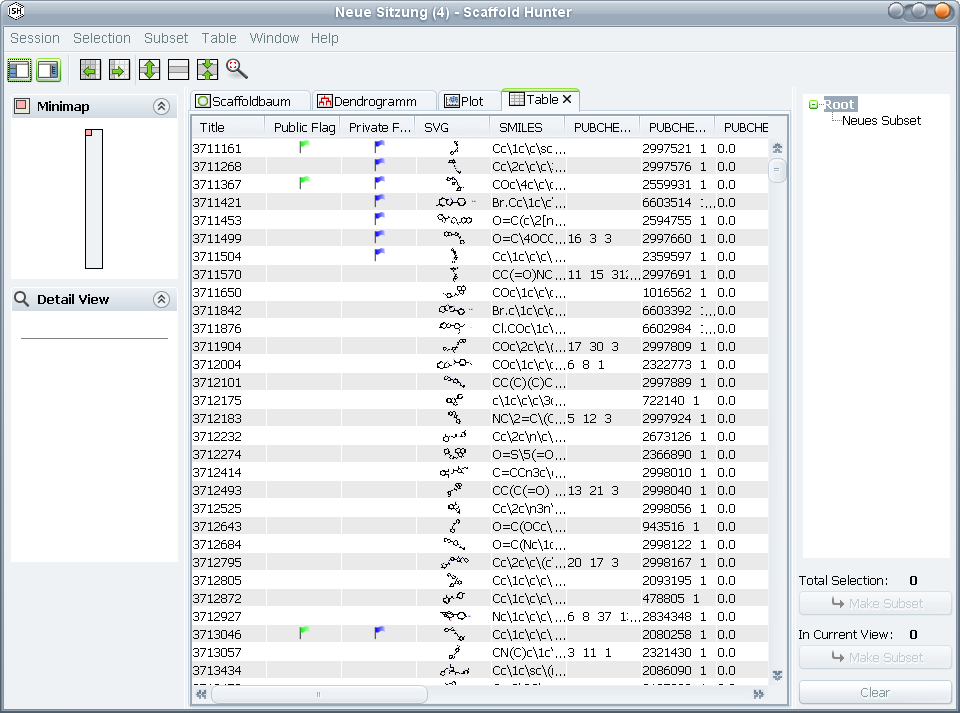
\includegraphics[width=0.8\columnwidth]{images/table/table_overview}
\par\end{centering}

\caption{The tableview}


%
\end{figure}



\subsection{Sorting and Ordering the Table}

When you open a table view the data is initially sorted by the molecule
title, but the sort order can be changed anytime by clicking on a
column header. The table view supports three sort criteria, which are
applied by consecutive clicks on column headers. The column selected last
gets the highest sort priority.

Apart from sorting the rows of the table you can reorder the columns
at any time by dragging them to their new position.


\subsection{Resizing Table Cells}

A table cell is often too small to show the information that it holds.
In this case three little dots appear at the end of the cell, to indicate
that the content is not completely shown. To address this problem there
are two ways to resize table cells: To change the width of a column
you can simply click on the right boundary line of the column header
and move it to the left or right, to make the whole column smaller
or wider. The height of the rows can be changed via three buttons
in the \tbar:
\begin{itemize}
\item 
\includegraphics{images/table/table_lines_enlarge} the
\textit{increase} button allows you to increase the number of text lines
that are shown in a table cell. Each time it is clicked one more line
is added.
\item 
\includegraphics{images/table/table_lines_shrink} the
\textit{decrease} button decreases the number of text lines per cell. 
\item 
\includegraphics{images/table/table_lines_normalize} the
\textit{normalize} button sets the number of text lines back to the
default value of one.
\end{itemize}
The content of a table cell is also shown in the \textit{Detail View}
panel in the \sbar, as soon as you move the mouse pointer to a cell.

%
\begin{figure}[!htb]
\begin{centering}
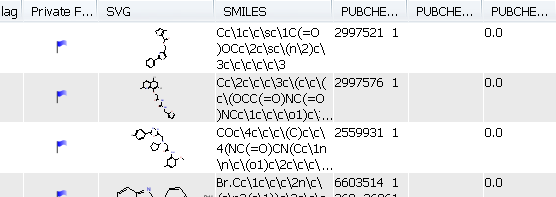
\includegraphics[width=0.8\columnwidth]{images/table/table_rowheight_example}
\par\end{centering}

\caption[Enlarged table rows]{Example of a table that shows three text lines in a table cell}


%
\end{figure}



\subsection{The Minimap}

The Minimap shows an abstract view of the complete table, where the
section that is currently shown in the main view is highlighted in
light red. Apart from just informative reasons the minimap can also
be used to scroll the table. Just click on the highlighted box and
drag it to another position.


\subsection{Sticky Columns}

When the table holds a lot of columns -- which is a very common case
-- then it is eligible that some columns are not scrolled horizontally
but stay visible the whole time. The molecule title column is an example;
it may be helpful if this column is always visible. This can be accomplished
by putting table columns into the \textit{sticky mode}: A sticky column
does not scroll horizontally. 

This feature can be accessed by two buttons in the \tbar:
\begin{itemize}
\item 
\includegraphics{images/table/table_sticky_add} A
click on this button turns the leftmost floating column (a column
which is not yet sticky) into the sticky mode. It will not scroll
horizontally anymore.
\item 
\includegraphics{images/table/table_sticky_remove} This
button turns the rightmost sticky column back into floating mode,
which means that the column will scroll as usual.
\end{itemize}
To indicate that a column is sticky it is shown a bit darker than
a normal, floating column.

%
\begin{figure}[!htb]
\begin{centering}
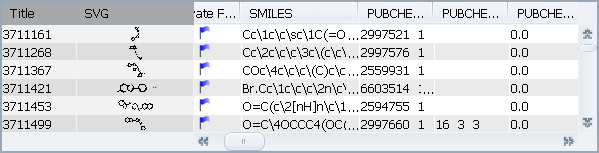
\includegraphics[width=0.8\columnwidth]{images/table/table_sticky_example}
\par\end{centering}

\caption[Sticky columns]{A table with two sticky columns. Note that the scrollbar at the bottom
does not include the sticky columns.}


%
\end{figure}



\subsection{Setting Flags}

Flags (public and private) can be set by using the context menu that
appears when you right-click anywhere in the table. The menu item ``Toggle
public flag (for \textit{molecule title})'' lets you toggle the public
flag for the specified molecule. The item ``Toggle private flag
(for \textit{molecule title})'' does the same for private flags. The
flags are shown in the table in separate columns.


\subsection{Selecting Molecules}

The selection of molecules (a row in the table) works slightly different
than with common tables. The only change we made is that the current
selection will not be cleared when you select a new molecule by clicking
on the corresponding row in the table. So you can select/unselect
multiple molecules by consecutive clicking on them.

Additionally you can select many molecules in a row when you hold
down the \texttt{Shift} key while clicking on the first and the last
molecule you want to select (which is the common behavior that you
may know from other programs).


\subsection{Writing and Editing Comments}

The comment editor for molecules can be opened by using the context menu. 


\subsection{Placeholders in Table Cells}

The table can be used to access all molecule information which is
stored in the database. To conserve memory these information are loaded
just when they should be shown. This may cause a little delay in
displaying the content of the table, which can be noticed at fast
scrolling over a long distance. During the loading process the table cells
are filled with three dots ({}``\ldots{}'') as placeholders. These
placeholders are replaced by the real content as soon as it is available.

  \section{Dendrogram}\label{sec:views:dendogram}
    The dendrogram view shows the result of a hierarchical clustering.
A hierarchical clustering works on a (sub)set of molecules and a couple of properties.
In the beginning, the clustering algorithm puts each molecule into one cluster. Then it searches for two molecules (clusters) with the smallest distance between each other based on the chosen properties.
When found, they are merged into a new cluster. 
This will be repeated until only one cluster remains.
The result is a tree which represents the merge history like shown in \figref{fig:dendrogram_tree}.

The dendrogram view shows this result, allows the user to navigate in the hierarchical tree structure and to highlight different clusters based on their relation.

\begin{figure}[!htb]
\centering
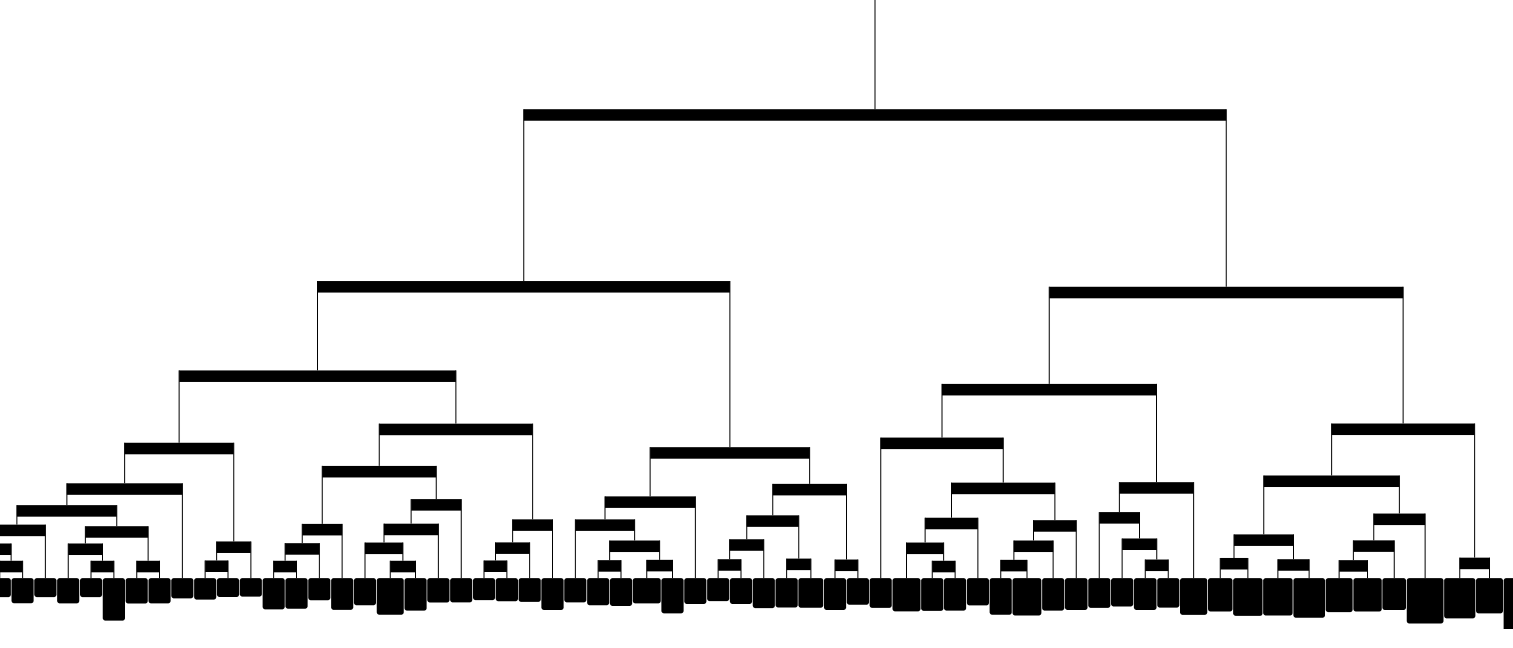
\includegraphics[width=1\textwidth]{images/dendrogram/dendrogram}
\caption{The tree frame}
\label{fig:dendrogram_tree}
\end{figure}

\subsection{The View in Detail}

The dendrogram view is separated in four parts, shown in \figref{fig:dendrogram_regions}. Each part is marked by a surrounding color as explained below:
\begin{itemize}
\item the tree frame in which the result is shown  (marked yellow)
\item the \sbar (marked red) 
\item the \tbar (marked blue)
\item a special representation of the table view (marked green)
\end{itemize}

 \begin{figure}[!htb]
\centering
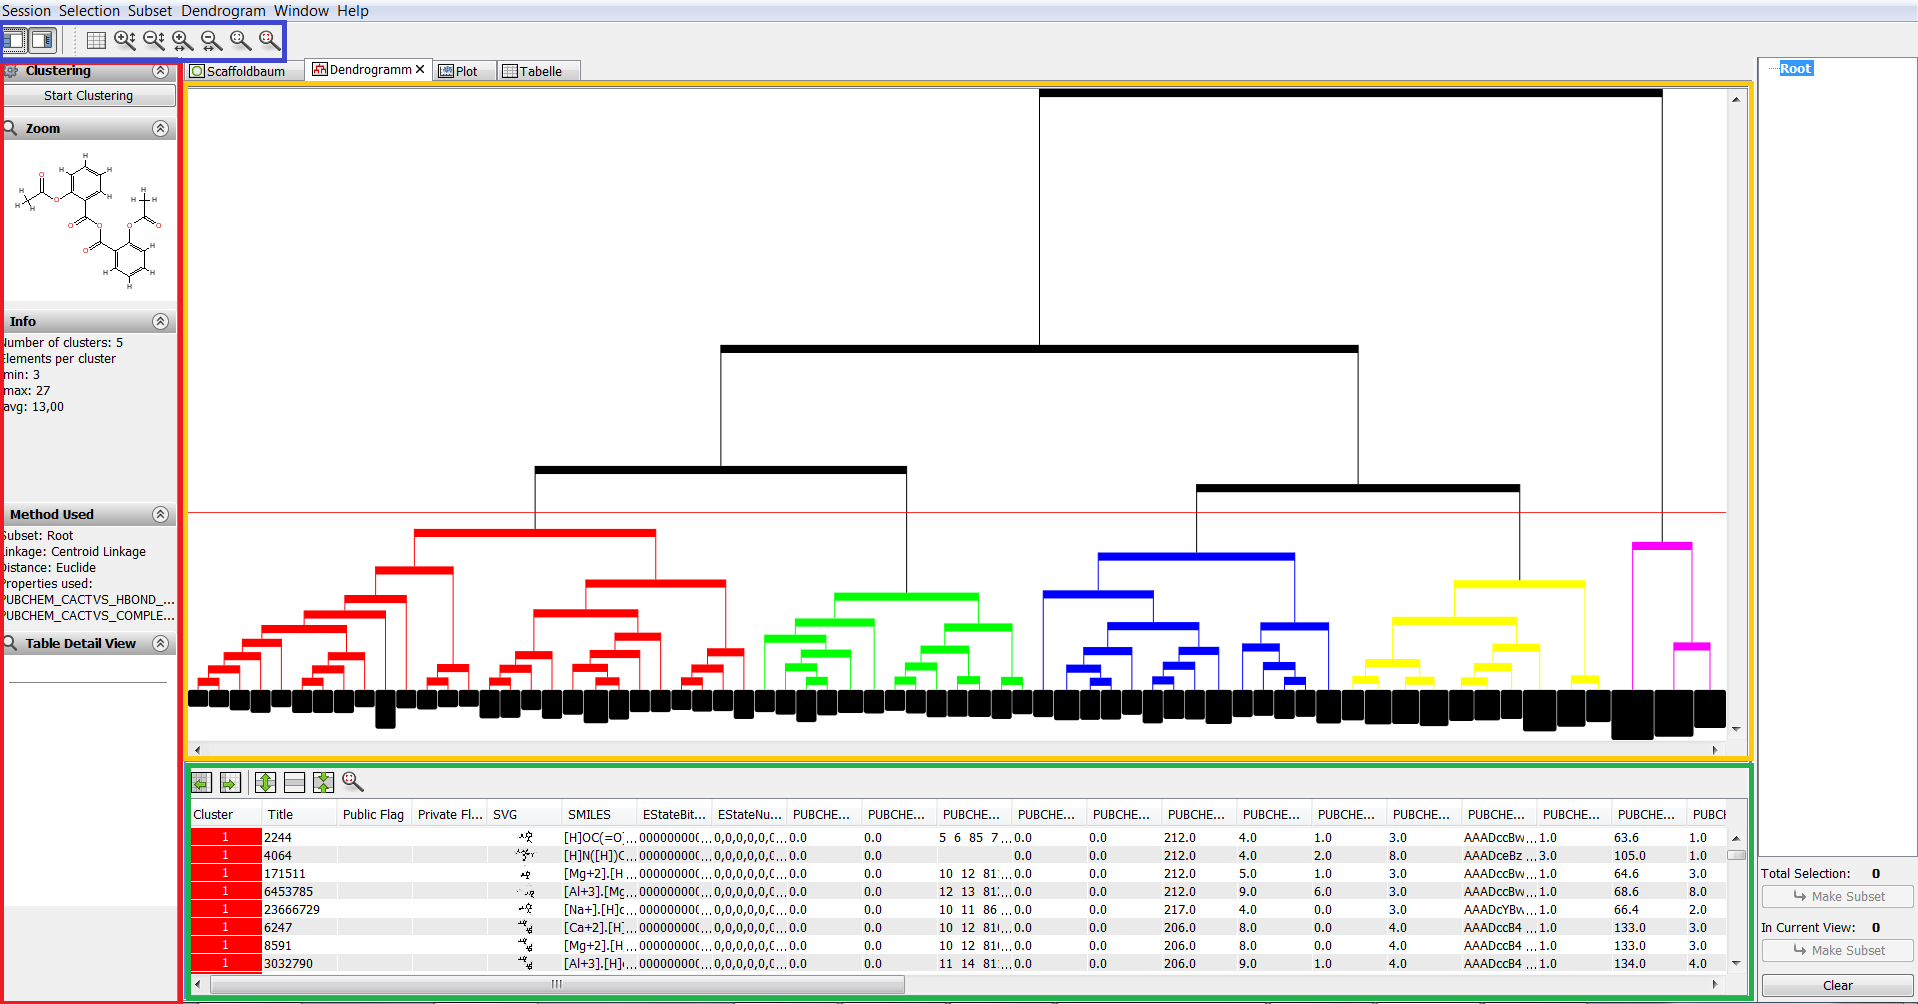
\includegraphics[width=1\textwidth]{images/dendrogram/overview_with_marks}
\caption{The whole view}
\label{fig:dendrogram_regions}
\end{figure} 

\subsection{Side Bar}

% \begin{figure}[!htb]
%\centering
%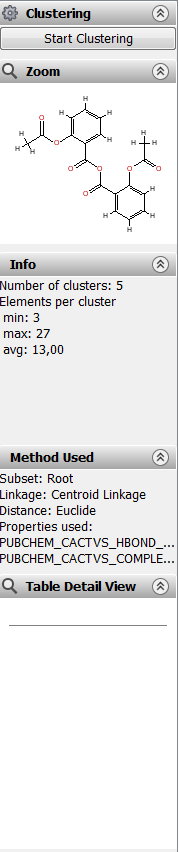
\includegraphics[width=0.1\textwidth]{images/dendrogram/sidebar}
%\caption{The Sidebar}
%\label{fig:dendrogram_sidebar}
%\end{figure} 
\figref{fig:dendrogram_regions} shows the dendrogram \sbar (marked red). 
\begin{itemize}
\item The \gui{Start Clustering} button opens the configuration dialog for the clustering
\item The \gui{Zoom} element shows the molecule under the mouse in detail
\item The \gui{Info} element shows statistical data about the currently chosen clustering
\item The \gui{Method Used} element shows which configuration was used to generate the actual dendrogram
\item The \gui{Table Detail} element is equal to its correspondent in the real table view
\end{itemize}



\subsection{Tree Frame} 

%\begin{figure}[!htb]
%\centering
%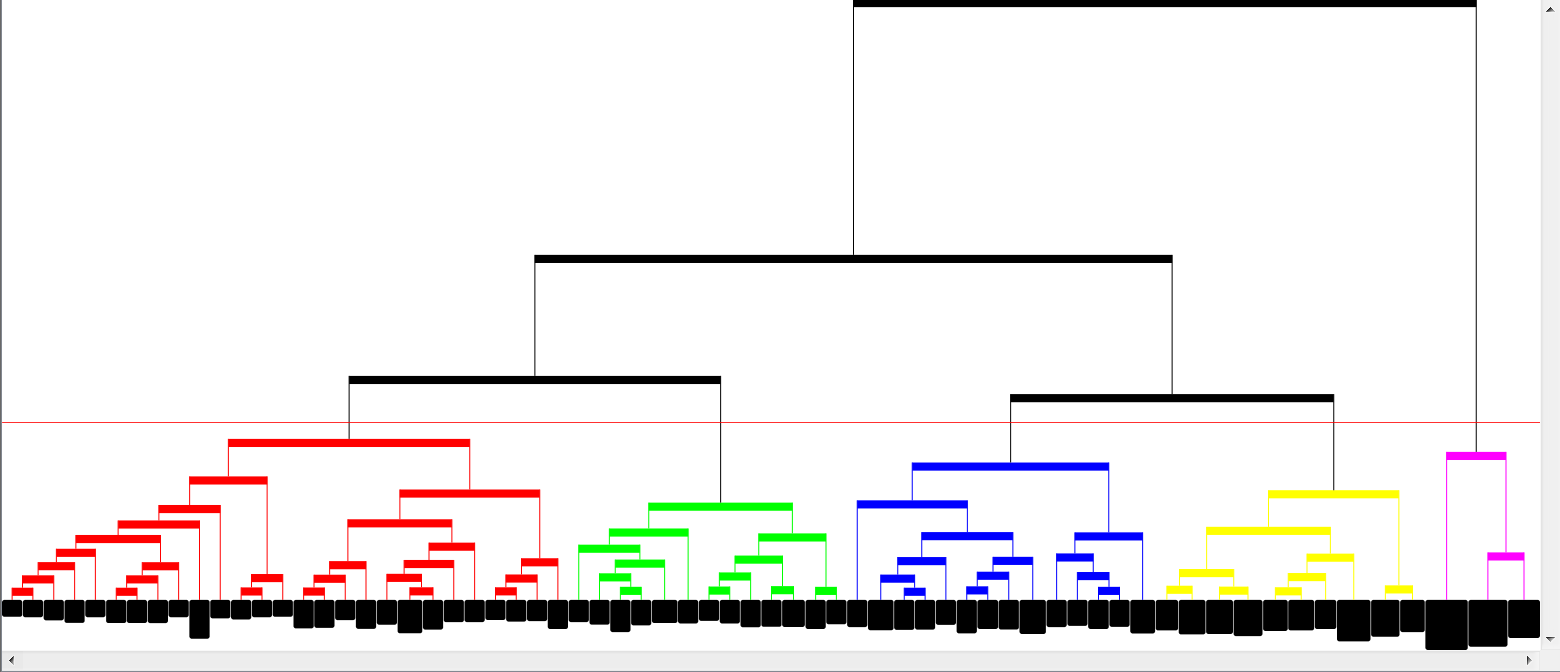
\includegraphics[width=0.8\textwidth]{images/dendrogram/main}
%\caption{The tree frame}
%\label{fig:dendrogram_tree}
%\end{figure}



In this part of the view you can see an actual dendrogram like shown in \figref{fig:dendrogram_tree}.
The molecules on the bottom are represented by black boxes because the zoom level is too small to show the real images.
The cluster selection bar shown in red in the middle is draggable and divides the subtrees below it into different clusters.
Each cluster separated this way is painted in a different own color.
The Info panel in the \sbar informs about the number of clusters created this way and their size.
With the mouse wheel or the keys “+” and “-“ the view can be zoomed in and out.
At a closer zoom level the black boxes at the bottom are replaced by the real molecule images like shown in \figref{fig:dendrogram_regions} (marked yellow). 

\begin{figure}[!htb]
\centering
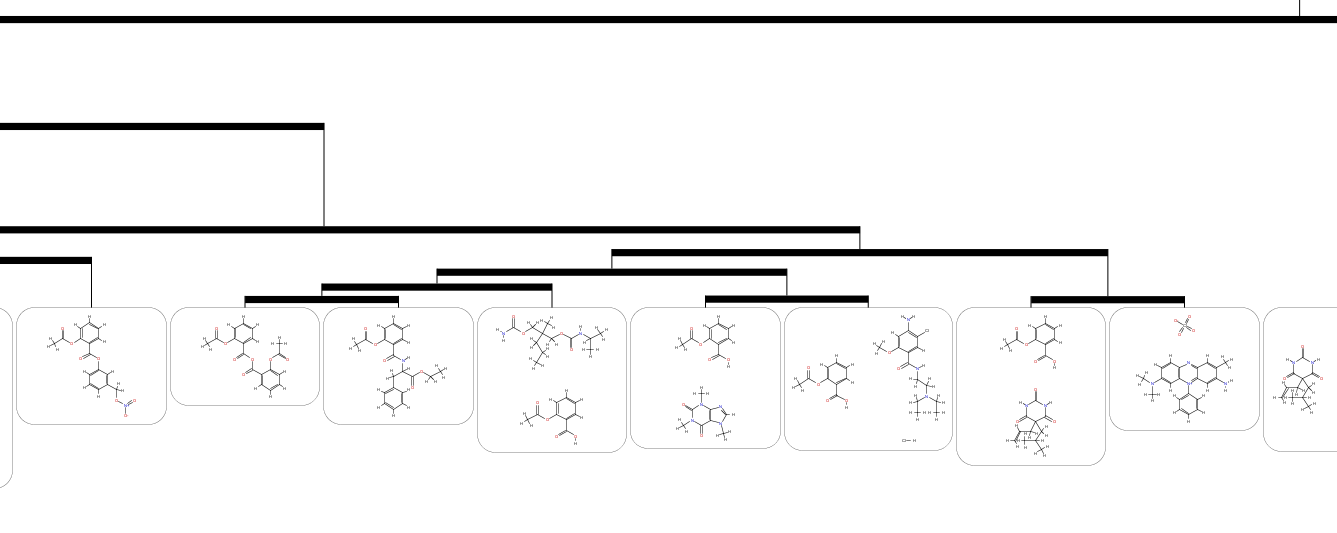
\includegraphics[width=0.8\textwidth]{images/dendrogram/zoomin}
\caption{Zoomed in}
\label{fig:dendrogram_zoom}
\end{figure} 

The zoom is separated into vertical and horizontal zoom.
This is necessary, because the tree usually has a very small height and a huge width.
So when zooming with the mouse wheel, the view scales the images and than adapts the tree above to fit in the window.
Zooming while holding the \texttt{Ctrl} key will scale only the tree, not the image. 
In addition to click on an image to add/remove it from the selection,
clicking on an inner node of the tree will result in selecting all leaves below it,
if at least one leaf is unselected and deselect them otherwise.


\subsection{Tool Bar}
 \begin{figure}[!htb]
\centering

\includegraphics[width=0.5\textwidth]{images/dendrogram/toolbar}
\caption{The \tbar}
\label{fig:dendrogram_tool}
\end{figure} 
The two buttons on the left shown in \figref{fig:dendrogram_tool} are the standard items to show/hide the side- and subset bar.
The third button  from the left shows/hides a special table below the dendrogram.
The next four buttons change the vertical and horizontal zoom of the dendrogram.
The second button from the right fits the dendrogram into the available space.
The button at the right zooms the view so that the whole selection is visible.


\subsection{Table}
% \begin{figure}[!htb]
%\centering
%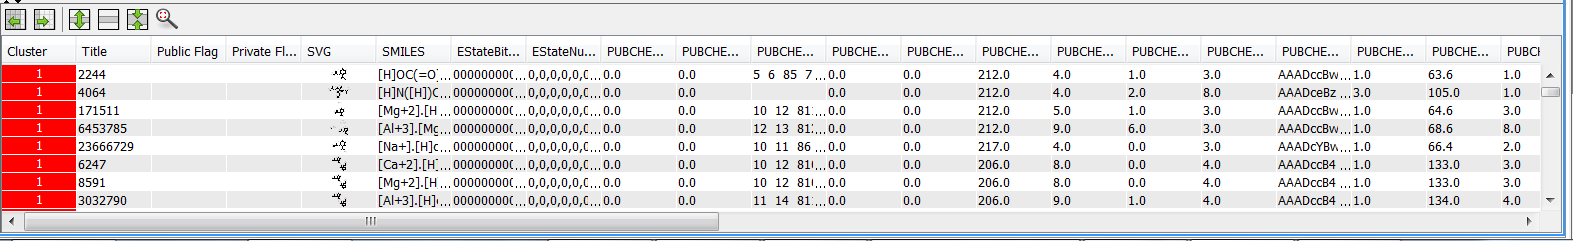
\includegraphics[width=1\textwidth]{images/dendrogram/table}
%\caption{The table below the dendrogram}
%\label{fig:dendrogram_table}
%\end{figure} 
The shown table below the dendrogram is the standard table view with one additional function, see \secref{sec:scaffoldhunter:table}.
The first column shows in which subclusters the selection bar in the dendrogram has divided the molecules.
An example is shown in \figref{fig:dendrogram_regions} (marked green).


\subsection{Clustering Configuration Panel}
\begin{figure}[!htb]
\centering
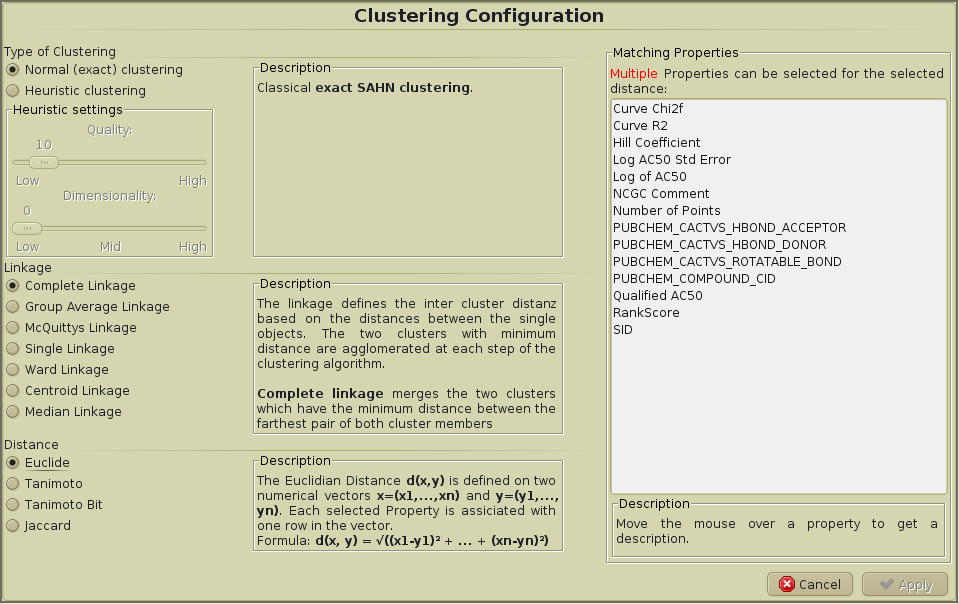
\includegraphics[width=0.9\textwidth]{images/dendrogram/clusteringConfig}
\caption{The clustering config dialog}
\label{fig:dendrogram_config}
\end{figure}
After clicking the start clustering button in the \sbar, a configuration panel as in \figref{fig:dendrogram_config} will show up.
Here, the user can choose from two clustering algorithms and select their parameters:

\subsubsection{Clustering Algorithms}
\paragraph{Normal (exact) clustering:} 
Classical exact SAHN clustering.

\warningbox{Warning}{The exact clustering can work on $2^{16}$ (65.536) molecules at a max, because of technical restrictions in Java and memory limitation.
Some of the parameters (\textit{Euclide} in combination with \textit{Ward, Median} or \textit{Centroid}) may work on more molecules, but this is experimental and should only be used with caution.
Please note that these restrictions do not apply to the heuristic algorithm.}

\paragraph{Heuristic clustering:} 
   The heuristic SAHN clustering algorithm should be 
   used if the runtime or the memory consumption by the exact clustering is to 
   high. Empiric tests showed that this algorithm can be considered useful for 
   subsets with a size larger that 10000 molecules. Two parameters are selectable:
   quality and dimensionality. Both have a direct influence on quality and speed.
   The dimensionality should be set according to the dimensionality of the data.
   Low for a dimensionality between 1 and 7, Mid 7-13 and High $>$ 13. If unsure
   start with a low dimensionality and use a higher value if the quality is 
   insufficient regardless of which quality is used.   


\subsubsection{Linkage \& Distance} \label{sec:scaffoldhunter:clustering:parameters}
The linkage method defines the way in which the distance between clusters is calculated and controls which pair should be merged.

\begin{itemize}

\item \textbf{Complete Linkage:} Merges the two clusters which have the minimum distance between the farthest pair of both cluster members.
\item \textbf{Group Average Linkage:} Merges the two clusters with the minimum distance of the unweighted cluster average (UPGMA).
\item \textbf{McQuittys Linkage}: Merges the two clusters with the minimum distance of the weighted cluster average (WPGMA).
\item \textbf{Single Linkage:} Merges the two clusters with the minimum distance between the nearest pair of both cluster members.
\item \textbf{Ward Linkage:} Merges the two clusters that lead to minimal variance increase.
\item \textbf{Centroid Linkage}: Merges the two clusters with the minimum distance of the unweighted centers (UPGMC).
\item \textbf{Median Linkage:} Merges the two clusters with the minimum distance of the weighted cluster centers (WPGMC).

\end{itemize}
The accepted types of properties depend on the distance computation.
\begin{itemize}

\item \textbf{Euclide:} Any number of numerical properties.
\item \textbf{Tanimoto:} Exactly one property which has to be a binary fingerprint.
\item \textbf{Tanimoto Bit:} Same as Tanimoto but works on bit strings not on character strings.
\item \textbf{Jaccard:} Works on one fingerprint property with feature counts on each position.
\end{itemize}


  \section{Plot}
    The plot view allows you to view numerical molecule data in form of
two- or three-dimensional scatterplots. Any numerical data that is
stored in the database can be displayed by linking them either to
one of the three spatial axes or to the color and size attributes
of a dot in the diagram.

%
\begin{figure}[!htb]
\begin{centering}
\includegraphics[width=0.8\columnwidth]{images/plot/plot_overview}
\par\end{centering}

\caption{The plot view}


%
\end{figure}



\subsection{Choosing the Data to be Displayed}

The first thing you want to do after opening a plot view is to select
the data that should be displayed. This can be done with the \textit{Property
Mapping} panel in the \sbar. Here you find a combo box for each of
the three spatial axes, for the dot color and the dot size, which allows
you to chose from numerical molecule properties. Additionally there is a slider
to apply a jitter to the data on the spatial axes.

%
\begin{figure}[!htb]
\begin{centering}
\includegraphics[width=0.3\columnwidth]{images/plot/property_mapping}
\par\end{centering}

\caption{The Property Mapping panel}
%
\end{figure}


Please note that the data has to be loaded from the database when
the mapping is changed. This can cause a slight delay before the diagram
is displayed. The mapping of data to axes is also shown in the \textit{Legend
panel} of the \sbar. There you can also see the domain of each
axis.


\subsection{Dot Color and Size}

The default color and size for dots can be changed at the \tbar.
These values are used when no data is mapped to the color/size properties.
As soon as you change the property mapping the elements in the \tbar
change to let you enter an interval for the color/size of the dots.

%
\begin{figure}
\begin{centering}
\includegraphics[width=0.3\columnwidth]{images/plot/dotcolor}
\par\end{centering}

\caption[Configuring dot colors]{The button for the color and the combo box for the dot size. The upper
figure shows the default behavior, when no data is mapped. The lower
figure shows the behavior when data is mapped to color/size.}
%
\end{figure}



\subsection{Hyperplanes}

Sometimes you do not want to see the complete set of data, but a small
part of it. This is where the concept of hyperplanes becomes useful.
Hyperplanes allow you to define thresholds for an axis, that means
a minimum and a maximum value that a data must have to be displayed
as dot in the diagram. They can be applied to any of the 5 dimensions (x,
y, z, color and size). When hyperplanes are set the associated threshold
values are shown in the diagram as black lines.

%
\begin{figure}[!htb]
\begin{centering}
\includegraphics[width=1.0\columnwidth]{images/plot/hyperplane_example}
\par\end{centering}

\caption[Use of hyperplanes]{The use of hyperplanes in a diagram: Without hyperplanes (left figure),
with hyperplanes at the y-axis (middle) and with the y-axis adjusting
to the hyperplanes (right figure).}


%
\end{figure}


Hyperplanes can be set and adjusted using the Hyperplanes panel in
the \sbar. For each of the 5 possible dimensions there is a slider that
lets you change the upper and the lower threshold value. For a better
control the values can also be entered as numbers in the text fields. 

%
\begin{figure}[!htb]
\begin{centering}
\includegraphics[width=0.18\columnwidth]{images/plot/hyperplane_panel}
\par\end{centering}

\caption{The hyperplane panel}
%
\end{figure}


While the axes always try to adjust themselves to the domain that
is mapped this behavior may be inappropriate when using hyperplanes.
By default a hyperplane does not influence the domain of an axis,
it just defines which values should be shown and which not. To let
an axis adjust according to the visible range that is defined by the
hyperplanes, click the checkbox for the axis in the panel.


\subsection{Zooming, Scrolling and Rotating the Diagram}

The diagram can be zoomed by using the buttons in the \tbar or by
using the mouse wheel. When using the mouse wheel the diagram will be
zoomed with keeping the focus at the current position of the mouse pointer.
Furthermore each axis can be scaled independently by using the buttons
in the Scale panel of the \sbar. In case the diagram becomes too
large to fit in the window you can scroll around by clicking in the
diagram with the left mouse button and drag it around. Rotating the
diagram works similar, just press the right mouse button while dragging.
Rotation only works in 3D-mode.

The \textit{Fit Graph} button in the \tbar always resets the zoom,
scroll position and rotation angles. Zooming and scrolling the diagram
to show the current selection can be done by clicking the button ``Zoom
to current selection'' in the \tbar.


\subsection{Highlighting, Selecting and Picking}

To avoid confusion with the dot colors the current selection and flags
(public and private) are not shown in the diagram by default. To make
them visible you have to set the accordant highlighting mode, which
can be done with the combo box in the \tbar. When the highlighting
mode is set to ``Selection'' then the dots that represent the
molecules in the current selection are shown in red. Setting the highlighting
mode to ``Public flag'' shows the molecules with a public flag
in green, while the highlighting mode ``Private flag'' shows the
molecules with a private flag in blue.

These features can also be set and removed from a molecule in the
plot view, according to Table~\ref{tableview mouse actions table}.

\begin{table}[!htb]
  \centering
  \begin{tabular}{p{0.3\columnwidth}p{0.55\columnwidth}}
  \textbf{Effect} & \textbf{Action}\\ \toprule
  add a molecule to or remove it from the selection & place the mouse pointer over the dot and click the left mouse button\\ \hline

  add multiple molecules to the selection & hold the \texttt{Shift} key and the left mouse button down while drawing a box
  around the dots\\ \hline

  remove multiple molecules from the selection & hold the \texttt{Ctrl} key and the left mouse button down while drawing a box
  around the dots\\ \hline

  toggle the public flag of a molecule & place the mouse pointer over the dot and click the middle mouse button\\ \hline

  toggle the private flag of a molecule & place the mouse pointer over the dot and click the middle mouse button
  while pressing the \texttt{Shift} key\\ \bottomrule
  \end{tabular}
  \caption{\Pview Mouse Actions}
  \label{tableview mouse actions table}
\end{table}



Please note that the highlighting mode adjusts automatically to the
action that is performed.

In any case, no matter if you perform one of these actions or not, the
molecule that belongs to the dot under the mouse pointer is shown in
the \textit{Detail View} panel in the \sbar.


\subsection{Hiding the Axis Ticks and Grids}

To toggle display of the axis ticks and grids there are two buttons
in the \tbar:
\begin{itemize}
\item \includegraphics{images/plot/plot_toggle_ticks} this
button toggles the display of the ticks
\item \includegraphics{images/plot/plot_toggle_grid}this
button toggles the display of the grids
\end{itemize}

  \section{Tree Map}
    The \tmview offers an alternative visualization of the scaffold tree, which is described in \subsecref{sec:scaffoldhunter:treegeneration}. The hierarchy defined by the scaffold tree is represented by nested rectangles, see \shortfigref{fig:treemap:example} for an example showing a small data set.

%
\begin{figure}[!htb]
\begin{centering}
\includegraphics[width=0.8\columnwidth]{images/treemap/treemap_example}
\par\end{centering}

\caption{Example of a tree map}
\label{fig:treemap:example}

%
\end{figure}

\subsection{TreeMap \& Tool Bar}

The treemap itself allows you to zoom and pan around to get a detailed view for all parts of the tree map. This navigation works similar to the \stview. For zooming you can either use the mouse wheel, the buttons in the tool bar or the \gui{TreeMap} menu. To move around you can left-click into the tree map and move your mouse while keeping the left mouse button pressed. When you right-click a node in the tree map, the camera is centered around this node, so that the node fills out the whole screen. The detail increases on small zoom levels showing the title and image of nodes.

\subsection{Property Mappings}\label{sec:treemap:propertymapping}

Initially the tree map is plotted without colors and a uniform size for every molecule. The size and color of all nodes can be changed by assigning chemical properties to them. \shortfigref{fig:treemap:sidebar:mapping} shows the \gui{Property Mapping} panel, which is used for this purpose.

%
\begin{figure}[!htb]
\begin{centering}
\includegraphics[scale=.6]{images/treemap/treemap_sidebar_mapping}
\par\end{centering}

\caption{Property Mapping panel}
\label{fig:treemap:sidebar:mapping}

%
\end{figure}

The individual options have the following functionality:

\begin{description}
\item[Node type] When \gui{Scaffolds} is selected only the scaffolds of the current subset are plotted. The option \gui{Molecules} additionally plots the molecules.
\item[Node size] Allows to map a chemical property to the node size. Only molecule properties can be mapped to the size, since the size of an inner nodes is always derived from its child nodes. Default is \gui{Nr of Molecules}.
\item[Node color] Allows to map a chemical property to the node color. The mapping can be combined with an accumulation function. This function works differently for molecule and scaffold properties:
\begin{itemize}
\item When using a molecule property, the accumulation function determines how to derive the colors of scaffolds from associated molecules. If \gui{Subtree cumulative} is enabled, the color of a scaffold is determined by the properties of all molecules that are contained in its subtree. If the option is disabled, only the molecules directly associated with the scaffold are considered.
\item When using a scaffold property and \gui{Subtree cumulative} is disabled, no accumulation is performed. If \gui{Subtree cumulative} is enabled, a scaffold combines its own color with its children's colors using the the function \gui{Acc.}.
\end{itemize}
If a property is not defined for a structure, it will be plotted in gray. 
\end{description}

\subsection{Color Legend}

The \gui{Legend} visualizes which property values have been mapped to which colors in the tree map. It is only visible, if a chemical property has been mapped to the node colors as explained in \subsecref{sec:treemap:propertymapping}. \shortfigref{fig:treemap:sidebar:legend} shows the legend for the tree map in \shortfigref{fig:treemap:example}.

%
\begin{figure}[!htb]
\begin{centering}
\includegraphics[scale=.6]{images/treemap/treemap_sidebar_legend}
\par\end{centering}

\caption{Color legend for the property mapping}
\label{fig:treemap:sidebar:legend}

%
\end{figure}

\subsection{Detail View}

The \gui{Detail View} shows additional information for a single scaffold or molecule. When you move the mouse cursor over a chemical structure in the tree map, an image and information about its size and color are displayed here.

%
\begin{figure}[!htb]
\begin{centering}
\includegraphics[scale=.6]{images/treemap/treemap_sidebar_detail}
\par\end{centering}

\caption{Detailed view for a single molecule}
\label{fig:treemap:sidebar:detail}

%
\end{figure}

\chapter{Export}
	Right clicking on a subset offers the possibility to export this subset. At the moment CSV and SDF export is supported. Starting the export will open the dialog shown in \figref{fig:export}.

\begin{figure}[!htb]
\centering
\includegraphics[width=0.4\textwidth]{images/sh_export_dialog}
\caption{Export Dialog}
\label{fig:export}
\end{figure} 

If CSV is chosen, the cell separator and the quotation character can be defined. After choosing the export format, the collection of properties which should be exported can be defined.
Clicking the export button will open a file chooser dialog to define the location and the name of the export.

After completing the export, the program will show a success message.


\bibliographystyle{plain}
\bibliography{literature}

\begin{appendix}

\chapter{Keyboard Shortcuts} \label{chap:scaffoldhunter:shortcuts}
  \begin{table}[ht]
  \centering
  \begin{tabular}{ccl}
					&	\textbf{Key}		& \textbf{Action} \\ \toprule
\multirow{3}*{\textbf{Zoom}}		&	+/-			& Zoom in/out \\
					&	0			& Fit graph / Table: Normalize rows\\
					&	s			& Fit selection / Table: Scroll to first selected molecule\\ \midrule
\multirow{6}*{\textbf{Selection}}	&	Ctrl+A			& Select all molecules/scaffolds\\
					&	Ctrl+Shift+A		& Deselect all molecules/scaffolds\\
					&	Ctrl+I			& Invert selection\\
					&	Ctrl+D			& Deselect all molecules in the current views subset\\
					&	Ctrl+N			& Make subset from selected molecules\\
					&	Ctrl+Shift+N		& Make subset from selected molecules in current view\\ \midrule
\multirow{5}*{\textbf{View}}		&	Ctrl+W			& Close current view\\
					&	Ctrl+PageUp		& Show next view\\
					&	Ctrl+PageDown		& Show previous view\\
					&	ALT+$\leftarrow$	& Toggle display of \sbar\\
					&	ALT+$\rightarrow$	& Toggle display of subset\\ \bottomrule
  \end{tabular}
  \caption{Global shortcuts (view-independent)}
\end{table}

\begin{table}[ht]
  \centering
  \begin{tabular}{ccl}
					&	\textbf{Mouse}					& \textbf{Action} \\ \toprule
\multirow{4}*{\textbf{Selection}} 	&	Left-click on molecule/scaffold			& Toggle selection of molecule/scaffold\\
					&	Shift + Left-click + Drag			& Select all molecules/scaffolds in selection rectangle\\
					&	Ctrl + Left-click + Drag			& Deselect all molecules/scaffolds in selection rectangle\\
					&	Left-click on tree node				& Toggle selection of subtree (\dview only)\\ \midrule
\multirow{2}*{\textbf{Flags}}     	&	Middle-click on molecule/scaffold		& Add/remove public flag for molecule/scaffold\\
					&	Shift + Middle-click on molecule/scaffold	& Add/remove private flag for molecule/scaffold\\ \midrule
\multirow{2}*{\textbf{Zoom}}		&	WheelUp / WheelDown				& Zoom in/out\\
					&	Ctrl + WheelUp / WheelDown			& Zoom in/out vertically (\dview only)\\ \midrule
\multirow{3}*{\textbf{Navigation}}	&	Left-click + Drag				& Move view area (\tview only)\\ 
					&	Right-click + Drag				& Rotate 3D-graph (\pview only)\\
					&	Right-click on molecule/scaffold		& Open context menu (all views; except \pview)\\ \bottomrule
  \end{tabular}
  \caption{Mouse actions (global and view-specific)}
\end{table}

\begin{table}[ht]
  \centering
  \begin{tabular}{ccl}
					&	\textbf{Key}		& \textbf{Action} \\ \toprule
\multirow{5}*{\textbf{Navigation}}	&	$\rightarrow$		& Move cursor clockwise \\
					&	$\leftarrow$		& Move cursor counter-clockwise \\
					&	$\uparrow$		& Move cursor to first child \\
					&	$\downarrow$		& Move cursor to parent \\
					&	C			& Focus cursor \\ \midrule
\multirow{3}*{\textbf{Radii}}		& 	Ctrl+$\uparrow$		& Increase radii \\
					&	Ctrl+$\downarrow$	& Decrease radii \\
					&	F			& Toggle radii lock \\ \midrule
\multirow{5}*{\textbf{Expanding}}	&	Enter			& Open/close children \\
					&	Ctrl+Enter		& Open/close entire subtree \\
					&	E			& Expand next level/Reduce to level \\
					&	Ctrl+E			& Expand all nodes \\
					&	Ctrl+Shift+E		& Reset to default expand level\\ \midrule
\multirow{4}*{\textbf{Visual}}		&	Space			& Select/deselect scaffold\\
					&	M	(pressed)	& Show molecules\\
					&	Ctrl+M			& Toggle permanent display of molecules\\
					&	Ctrl+P			& Configure property mappings...\\ \midrule
\multirow{7}*{\textbf{Node scaling}}	&	PageUp			& Scale up cursor scaffold \\
					&	PageDown		& Scale down cursor scaffold \\
					&	Alt+PageUp		& Scale up selected scaffolds \\
					&	Alt+PageDown		& Scale down selected scaffolds \\
					&	N			& Normalize cursor scaffold \\
					&	Alt+N			& Normalize selected scaffolds\\
					&	A			& Normalize all nodes\\ \hline
%		      T    ??? does not exist any longer                      & Toggle tooltip \\
\multirow{3}*{\textbf{Layout}}		&	L			& Switch to linear layout\\
					&	B			& Switch to balloon layout\\
					&	R			& Switch to radial layout\\ \bottomrule
  \end{tabular}
  \caption{\Stview shortcuts}
\end{table}

\begin{table}[ht]
  \centering
  \begin{tabular}{cl}
    \textbf{Key}	& \textbf{Action} \\ \toprule
    Ctrl+G		& Toggle display of grid \\
    Ctrl+T		& Toggle display of ticks \\ \bottomrule
  \end{tabular}
  \caption{\Pview shortcuts}
\end{table}

\begin{table}[ht]
  \centering
  \begin{tabular}{cl}
    \textbf{Key}	& \textbf{Action} \\ \toprule
    Ctrl+T		& Toggle display of table \\
    Ctrl + Plus		& Zoom in vertically \\
    Ctrl + Minus	& Zoom out horizontally\\ \bottomrule
  \end{tabular}
  \caption{\Dview shortcuts}
\end{table}

\chapter{How to Write Plugins} \label{chap:scaffoldhunter:writeplugins}
In this chapter you will learn the basic parts needed to write new plugins.
Feel free to write new import or calc plugins or to expand the existing ones.
We are always happy to get new plugin (versions) submitted.

    \section{Import Plugins}
      \subsection{What is needed to write a new import plugin}
To write a new import plugin you need the \sh source code. The plugins basis is held in the \javapackage{edu.udo.scaffoldhunter.plugins.dataimport}. You should put every new plugin inside the \javapackage{edu.""udo.""scaffoldhunter.""plugins.""dataimport.""impl.""PLUGINNAME} package.

\subsection{Basic parts of a plugin}
Every import plugin consists of three base classes:

\paragraph{PluginSettingsPanel}
At first a class on base of \javaclass{PluginSettingsPanel}. This is a \javaclass{JPanel} which shows the configuration options of the plugin in the Import Dialog. It has methods to get and set the current configuration options and those which have been set in the past.

\paragraph{PluginResults}
The \javaclass{PluginResults} are built on base of a plugin run and contain all results of the specific plugin with a given configuration. At first there are some basic results, such as the number of results, name of the rows in resulting data, which of those rows maybe numeric, and finally iterables consisting of the molecules.

\paragraph{ImportPlugin}
The import plugin itself is the interface to \sh. It gives instances of the \javaclass{PluginSettingsPanel} and the \javainterface{PluginResults} back, has a method to test if a configuration will give useable results or fail in the beginning and has some basic information, as name and an UID.

Next to those classes there are the \javaclass{Arguments}, which is a simple \javaclass{Object} consisting of a current configuration and a class implementing the \javainterface{Serializeable} interface which contains data, which is saved into the database. It could be used to save older settings.

\subsection{Writing a simple plugin}
The source tree already consists of a very simple plugin, it is named \javaclass{DummyImportPlugin}. In this part you will get a step by step guide whose result will be such a simple plugin, which can generate a simple error message and gives two empty molecules back.

\subsection{First Version - An empty configuration panel}
The source of the first version can be found in the \javapackage{edu.""udo.""scaffoldhunter.""plugins.""dataimport.""impl.""example1} package. This example contains everything that is needed to be listed in the Import Dialog. With this example you are not able to go further through the import process, it does not give back all needed parts. Lets look at the important parts of the source.

\subsubsection{ImportPlugin.java}
\paragraph{@PluginImplementation}
The first important thing is the Annotation \javaannotation{@PluginImplementation}. This is needed by the used plugin framework to recognize this class as a plugin. If this line is missing, the plugin will not be listed in the import dialog.

\paragraph{extends AbstractImportPlugin}
Your import plugin has to inherit from \javaclass{AbstractImportPlugin}. If instead of this you only go and implement the \javainterface{ImportPlugin} interface there will be a wrong name in the list of import sources in the import dialog.

\paragraph{getTitle()}
The \javamethod{getTitle()} method returns a short name of the plugin. This is also the name which is listed in the import dialog.

\paragraph{getID()}
In \javamethod{getID()} your plugin should return a unique name of the plugin, this is for example used by \sh to match saved properties for the plugins. During the development process of \sh all Plugins used the form      \verb+CLASSNAME_VERSION+ that should be unique enough.

\paragraph{getDescription()}
The \javamethod{getDescription()} method returns a description about for what the import plugin can be used, like "This is an import plugin which can be used to import data from our internal webfrontend".

\paragraph{getSettingsPanel(settings,arguments)}
Here we return only an empty \javaclass{SettingsPanel}. This will change in the third example.

\paragraph{getResults(arguments)}
In the first example we don't have a result object yet.

\paragraph{checkArguments(arguments)}
Inside of the \javamethod{checkArguments(arguments)} method you should check if a plugin run will definitely fail, then you return an error message, otherwise null. In this example we return a message to interrupt the import process. Otherwise the Example1 plugin would cause errors in the future.


\subsection{Second Version - We give a simple result}
In the second step we will add an \javaclass{ImportPluginResult} object, which will give back one molecule without a structure but with two properties (one will be numerical).

\subsubsection{Example2ImportPluginResults.java}
As a new part in the second Example we have a \javaclass{PluginResults} class. This class has to implement the \javainterface{PluginResults} interface. Let us go through the new methods.

\paragraph{getSourceProperties()}
In the \javamethod{getSourceProperties()} method you have to give back a Map of \javaclass{PropertyNames}. The Map can also include \javaclass{PropertyDefinitions}, which  could build the base for a more detailed way of defining the type of the property, which should be implemented in further versions of \sh, most times a null-value for the \javaclass{PropertyDefinition} part is sufficient. So we generate a new Set with the two property names "title" and "number".

\paragraph{getProbablyNumeric()}
The \javamethod{getProbablyNumeric()} method gives back a Set of strings containing the property names of those properties which contain numeric values. It is used in the mapping dialog to automatically select which properties should be treated as numbers. In this example it is the property "number".

\paragraph{getMolecules()}
This method contains the main plugin task. It returns the \javainterface{Iterable} which contains the new molecules. Here we create a No Notifying Molecule (\javaclass{NNMolecule}). The usage of \javaclass{NNMolecule} in place of \javaclass{Molecule} has a very high positive impact on the import speed. We add our two properties to the molecule and put it into a simple List which we return. When you write your own plugin you will probably write your own class implementing the \javainterface{Iterable} interface.

\paragraph{getNumMolecules()}
The \javamethod{getNumMolecules()} method returns the number of molecules which will be imported. We built one \javaclass{Molecule} so we return 1.

\paragraph{addMessageListener(listener), removeMessageListener(listener)}
The \javamethod{add/removeMessageListener} methods will be used to give fault messages during the import process, so we just ignore them now.

\subsubsection{Example2ImportPlugin.java}
In the plugin itself there are only small changes.

\paragraph{getResults(arguments)}
The created \javainterface{PluginResults} implementation is returned.

\paragraph{checkArguments(arguments)}
We return something, so do not generate an error message and return null.


\subsection{Third Version - Settings panel}
The third example adds a very simple Settings Panel to the plugin where we can type in the molecule title and an error message for the \javamethod{checkArguments(arguments)} method.

\subsubsection{Example3PluginArguments.java}
At first there is a new Class, \javaclass{Example3PluginArguments}, which holds the arguments for a single plugin run. This is a very simple class with three fields:
\begin{itemize}
  \item \javatype{boolean} error : Will be true, if the plugin should generate an error message in the \javamethod{checkArguments} method.
  \item \javaclass{String} errorMessage : The message which will be given back if the plugin generates an error message.
  \item \javaclass{String} moleculeTitle : The content of the title property in the molecule.
\end{itemize}

\subsubsection{Example3PluginSettingsPanel.java}
The second new class is the \javaclass{Example3PluginConfigurationPanel}. So we are able to fill the configuration panel within the import dialog with content.

\paragraph{Example3PluginSettingsPanel(arguments)}
The constructor first checks if the ConfigurationPanel got an arguments object, this happens when you select an item in the import jobs list of the import dialog. If it does not get an \javaclass{Example3PluginArguments} object it generates a new one with the default values. Afterwards the different parts of the Panel are generated, with the values from the arguments object and then some formatting is done.

\paragraph{getSettings()}
We do not safe any settings, so this method returns null. If you want to have saveable settings generate a new class that implements \javainterface{Serializeable} which holds those settings. An instance of this class with the content which should be saved has to be returned here.

\paragraph{getArguments()}
The \javamethod{getArguments()} method returns the current settings being made in a \javaclass{Example3PluginArguments} object. So here we read the \javaclass{JCheckBox} state, and the content of the two \javaclass{JTextField} instances and put them to the corresponding fields in the returned object.


\subsubsection{Example3ImportPluginResults.java}
In the Results class we only had to add the arguments and built the molecule title property on it.
So first there is a new private field \javaclass{Example3ImportPluginArguments} which holds the arguments for the plugin run.

\paragraph{Example3ImportPluginResults(arguments)}
The new constructor just sets the internal arguments field to the supplied arguments. When you write a plugin you should put some initialization here, like opening database connections, counting of molecules, etc.

\paragraph{getMolecules()}
In the \javamethod{getMolecules()} method we set the title property according to the \javavar{moleculeTitle} field in the arguments.

\subsubsection{Example3ImportPlugin.java}

\paragraph{getSettingsPanel(settings,arguments)}
Here our new \javaclass{SettingsPanel} is returned and we cast the arguments into the right type.

\paragraph{getResults(arguments)}
Same for the results, they now await arguments, so the class gets them.

\paragraph{checkArguments(arguments)}
Now we are able to check, if a plugin run will "succeed" so we either give the error message from the arguments if the user wants it or return null.

\subsection{Fourth and last version - Output a message during the import}
At this point you are able to build configurations, check for an error at the beginning of the import and return molecules. There is only one last part missing, the possibility to send Messages during the import. This is realized in the \javaclass{Example4ImportPlugin}.

\subsubsection{Example4ImportPluginArguments.java}
At first we added a new configuration option to switch the message on or off. It is named \javavar{generateMessage}.

\subsubsection{Example4ImportPluginSettingsPanel.java}
In the Settings panel the default value for the \javavar{generateMessage} is added. Furthermore there is a \javaclass{JCheckBox} added, to switch the Message on or off.

\subsubsection{Example4ImportPluginResults.java}
In the \javaclass{Example4ImportPluginResults} some changes have been made. First there is a LinkedList which holds the listeners which are registered with the results.

\paragraph{addMessageListener(listener)}
The \javamethod{addMessageListener(listener)} method now adds the given listener to the \javavar{messageListeners} list.

\paragraph{removeMessageListener(listener)}
The \javamethod{removeMessageListener(listener)} method now removes the given listener from the \javavar{messageListeners} list.

\paragraph{getMolecules()}
The \javamethod{getMolecules()} method has been rewritten. Instead of a simple List it now returns a self written \verb+Iterable<Molecule>+, which still gives back our simple Molecule. But in the \javamethod{getNext()} method of the included \verb+Iterator<Molecule>+ the argument generateMessage is checked and if we should send a Message a new instance of the type \javaclass{edu.udo.scaffoldhunter.model.data.Message} is generated which consists of a Message saying that the Molecule structure on base of a SMILES string could not be generated.
You only need to give a type of the message to the constructor of the message, the name can be empty and the other two arguments null, they are set in other parts of the import process. Some MessageTypes are already  defined in the \javaclass{edu.udo.scaffoldhunter.model.dataimport.MergeMessageTypes} class. Two of them should be useful for import plugins:\\
\begin{table}[!htb]
  \begin{tabular}{ll}
    \textbf{Name}	& \textbf{Description}\\ \toprule
    \verb+MOLECULE_BY_SMILES_FAILED+	& Can't build Molecule on base of SMILES\\ \midrule
    \verb+MOLECULE_BY_MOL_FAILED+	& Can't build Molecule on base of MOL\\ \bottomrule
  \end{tabular}
\end{table}
If you need other MessageTypes just implement them using the MessageType interface.
    
    \section{Calculation Plugins}
      \subsection{What is needed to write a new calculation plugin}
To write a new calc plugin you need the \sh source code.
The calc plugin interfaces and helper classes are stored in the following packages:

\begin{itemize}
  \item \javapackage{edu.udo.scaffoldhunter.plugins}
  \item \javapackage{edu.udo.scaffoldhunter.plugins.datacalculation}
  \item \javapackage{edu.udo.scaffoldhunter.model.data}
  \item \javapackage{edu.udo.scaffoldhunter.model.datacalculation}
\end{itemize}

Your plugin should be placed in a new package called
\javapackage{edu.""udo.""scaffoldhunter.""plugins.""datacalculation.""impl.""PLUGINNAME},
where PLUGINNAME should be replaced by the name of your plugin.

\subsection{Basic parts of a plugin}
Every import plugin consists of three base classes:

  \paragraph{PluginSettingsPanel}
  At first a class on base of \javaclass{PluginSettingsPanel}
  from \javapackage{edu.""udo.""scaffoldhunter.""plugins}.
  This is a \javaclass{JPanel} which shows the configuration options of the plugin
  in the \guidialog{Calc Dialog} (See \figref{fig:createcalcjobdialog}).
  It has methods to get and set the current configuration options
  and those which have been set in the past.

  \paragraph{CalcPluginResults}
  The \javaclass{CalcPluginResults} class is constructed during a plugin run
  and contains all results of the specific plugin with a given configuration.
  With help of the \javaclass{CalcPluginResults} class the calc plugin
  tells the plugin system which properties where calculated and
  supplies an \javainterface{Iterable} over all molecules
  (the calculated properties are attached to those molecules).

  \paragraph{CalcPlugin}
  The calc plugin itself is the interface to \sh.
  It returns instances of the \javaclass{PluginSettingsPanel}
  and the \javainterface{CalcPluginResults},
  has a setter method to get notified about existing properties and
  has getter methods which provide basic information like the title,
  description and unique identifier of the plugin.\\

  Next to those classes there is a \javaclass{PluginArguments} class,
  which is a simple \javaclass{Object} representing a plugin configuration
  and a \javaclass{CalcPluginSettings} class implementing
  the \javainterface{Serializable} interface which contains data,
  that is saved into the database.
  It could be used by the plugin to save and retrieve
  settings like e.g. an arguments history.

\subsection{Writing a simple plugin}
In the next sections we will -- in a step-by-step guide --
develop a plugin that reads an existing numerical property,
adds or subtracts 1.0 from the property
and saves the new value into a new property.
The plugin is configurable and has the ability
to send messages to the GUI if something goes wrong.

\subsection{First version - Create a plugin that does nothing}
The first plugin version can be found in
\javapackage{edu.""udo.""scaffoldhunter.""plugins.""datacalculation.""impl.""example1}.
It implements just the basic things, while having no real functionality.
It can be selected and executed, but behaves transparently,
thus doesn't calculate anything.

  \subsubsection{Example1CalcPlugin.java}

    \paragraph{@PluginImplementation}
    The first important thing is the \javaannotation{@PluginImplementation}
    annotation above the class definition.
    This is needed by the plugin framework to recognize this class as a plugin.
    If this line is missing, the plugin will not be listed in the calc dialog.

    \paragraph{extends AbstractCalcPlugin}
    Your calc plugin has to inherit from \javaclass{AbstractCalcPlugin}.
    This abstract class implements the \javainterface{ImportPlugin} interface
    for you and also overrides the \javamethod{toString()} method so that your plugin title
    is shown correctly in the list of calc plugins in the calc dialog.

    \paragraph{getTitle()}
    The \javamethod{getTitle()} method returns a short name of the plugin.
    This is also the name which is listed in the calc dialog.

    \paragraph{getID()}
    In \javamethod{getID()} your plugin should return a unique name of the plugin,
    this is for example used by \sh to match saved properties for the plugins.
    During the development process of \sh all plugins used
    the form \verb+CLASSNAME_VERSION+ that should be unique enough.

    \paragraph{getDescription()}
    The \javamethod{getDescription()} method returns a description
    about for what the calc plugin can be used,
    like "This is a calc plugin which can be used to calculate the xyz-fingerprint".

    \paragraph{setAvailableProperties(availableProperties)}
    As we do not need to know something about existing properties yet,
    we leave this method blanc.
    This will change in the fourth version.

    \paragraph{getSettingsPanel(settings,arguments)}
    As we do not need any configuration yet,
    we just return an empty instance of \javaclass{SettingsPanel}.
    This will change in the third version.

    \paragraph{getResults(arguments,molecules,msgListener)}
    The given \javavar{molecules} parameter is
    an \javaclass{Iterable} over the available molecules.
    As we do not want to calculate any property nor modify any molecule,
    we return a class implementing \javainterface{CalcPluginResults} interface,
    which will return the \javavar{molecules} parameter unchanged.
    It also returns an empty \javaclass{Set} of \javaclass{PropertyDefintition}s,
    which declares we have no properties to be added to \sh.

\subsection{Second version - 'Calculate' a new property}
The second version of the plugin can be found in
\javapackage{edu.""udo.""scaffoldhunter.""plugins.""datacal""culation.""impl.""example2}.
Here, we change our last plugin version,
so that it creates and saves a property for all given molecules.
We don't really calculate something,
we just create a numerical property with value 1.0.

  \subsubsection{Example2CalcPlugin.java}
    \paragraph{Example2CalcPlugin()}
    In the constructor of \javaclass{Example2CalcPlugin},
    we create a new \javaclass{Property""Definition}
    and store it in a member variable named \javavar{propDef}.
    \javavar{propDef} describes the characteristics of the property we want to add to every molecule.
    Therefore we set the property type to be a numerical property.
    See \tableref{Table:scaffoldhunter:calc:PropertyType} to learn which property types are available.
    We also set a title, a description and a key.
    The title is a short description of the property,
    where as the description is a sentence describing the property in detail.
    The property key is used for internal processing and written in uppercase letters by convention.
    It should be as unique as possible.
    Additionally, we set the property definition to be mappable
    (this means it can be mapped on a visual feature in the main program)
    and define it as molecule property (by saying it is not a scaffold property).

    \begin{table}[!htb]
      \begin{tabular}{cp{10cm}}
	\textbf{PropertyType}	& \textbf{Description} \\ \toprule
	\verb+NumProperty+		& An ordinary numerical property.\\ \midrule
	\verb+StringProperty+	& An ordinary string property.\\ \midrule
	\verb+BitStringFingerprint+	& A bit fingerprint represented by a string of 1 and 0 (chars).\\ \midrule
	\verb+BitFingerprint+	& A bit fingerprint that interprets every bit of a string as a bit. This is logically identical to BitStringFingerprint but has less memory consumption.\\ \midrule
	\verb+NumericalFingerprint+	& A fingerprint that consists of many numerical values. A NumericalFingerprint is a simple string with integer values separated by a comma: int,int,...\\ \bottomrule
      \end{tabular}
      \caption{Property Types}
      \label{Table:scaffoldhunter:calc:PropertyType}
    \end{table}

    \paragraph{getResults(arguments,molecules,msgListener)} \label{sec:scaffoldhunter:calc:Example2CalcPlugin.java:getResults}
    Here we change our custom \javaclass{CalcPluginResults} implementation:
    In the \javamethod{getMolecules()} method we not simply return the \javaclass{Iterable} over the available molecules like in the last version.
    Instead we transform all molecules with a custom transform function first, and return the transformed molecules.
    The transform function will do all the work like calculating a property and adding it to the molecule.
    Read \subsecref{sec:scaffoldhunter:calc:Example2CalcPluginTransformFunction.java} to see what is does in our example.\\
    In the \javamethod{getCalculatedProperties()} method we return a \javaclass{Set} which contains the \javavar{propDef} we created before.
    This notifies the plugin system we want to add this property.

  \subsubsection{Example2CalcPluginTransformFunction.java} \label{sec:scaffoldhunter:calc:Example2CalcPluginTransformFunction.java}

    \paragraph{implements Function$<$Molecule, Molecule$>$}
    Our transform function needs to implement the \javainterface{Function} interface
    and we want to transform from molecule to molecule.

    \paragraph{Example2CalcPluginTransformFunction(propDef)}
    In the constructor of the \javaclass{Example2""Calc""Plugin""Transform""Function} we simply save the given
    \javaclass{PropertyDefinition} parameter in a member variable named \javavar{propDef}.
    We will need this in the \javamethod{apply()} function.

    \paragraph{apply(molecule)}
    The \javamethod{apply()} functions gets one molecule as input parameter, and returns the transformed molecule.
    We just insert a mapping from the \javavar{propDef} (our \javaclass{PropertyDefinition}) to the value $1.0$ to the molecules property map.
    Then we return the molecule. The plugin system will read this map and save the property.

\subsection{Third version - Make the plugin configurable}
The third version of the plugin can be found in
\javapackage{edu.""udo.""scaffoldhunter.""plugins.""datacalculation.""impl.""example3}.
We now want to make the plugin configurable.
The user should choose whether the 'calculated'/added property is set to $1.0$ or $-1.0$, by enabling or disabling a checkbox.
Therefore we will extend \javaclass{PluginSettingsPanel} by a checkbox
and introduce a \javaclass{CalcPluginArguments} class to store the state of the checkbox.
  
  \subsubsection{Example3CalcPluginArguments.java}
  The \javaclass{Example3CalcPluginArguments} class just has a
  \javatype{boolean} member variable encoding the state of the checkbox.
  Additionally it has a getter and a setter method for this variable.

  \subsubsection{Example3CalcPluginSettingsPanel.java}
    \paragraph{Example3CalcPluginSettingsPanel(arguments)}
    The \javaclass{Example3CalcPluginSettingsPanel}s constructor saves
    a reference to the given \javavar{arguments} parameter.
    It also creates a checkbox which is initialized to the state stored
    in the \javavar{arguments} parameter and adds it to the panel.
    Additionally it creates an \javainterface{ActionListener} which reacts on changes
    of the checkbox state and updates the corresponding
    \javatype{boolean} value in the \javavar{arguments}.

    \paragraph{getArguments()}
    The \javamethod{getArguments()} method simply returns the \javavar{arguments}.

  \subsubsection{Example3CalcPluginTransformFunction.java}
  The \javaclass{Example3CalcPluginTransformFunction} constructor is changed
  so that it saves a reference to the new \javavar{arguments} parameter.

    \paragraph{apply(molecule)}
    The \javamethod{apply()} method now determines the property value based on the saved \javavar{arguments}.

  \subsubsection{Example3CalcPlugin.java}
      In the calc plugin itself there are just a few changes. The following methods changed:

      \paragraph{getSettingsPanel(settings,arguments)}
      The \javamethod{getSettingsPanel()} method creates
      a new \javaclass{Example3""CalcPlugin""Arguments} instance,
      if the \javavar{arguments} parameter is \javatype{null}.
      You should always initialize your arguments in this way.
      Afterwards a new \javaclass{Example3""CalcPlugin""SettingsPanel} is
      instantiated with the \javaclass{Example3""CalcPlugin""Arguments} as parameter and returned.

      \paragraph{getResults(arguments,molecules,msgListener)}
      In the \javamethod{getResults()} method there is just one small change:
      The \javavar{arguments} parameter is casted and passed
      to the \javaclass{Example3""CalcPlugin""Transform""Function}s constructor.

\subsection{Fourth version - Use existing properties for calculation}
The fourth version of the plugin can be found in
\javapackage{edu.""udo.""scaffoldhunter.""plugins.""datacalculation.""impl.""example4}.
In this version we want to read existing numerical properties and let the user select one.
For every molecule our plugin creates a new property which is the
same as the selected one, but $1.0$ or $-1.0$ (based on the users choice) is added to the property value.

  \subsubsection{Example4CalcPluginArguments.java}
  A new variable which saves the property chosen by the user is added together
  with corresponding getter and setter methods
  to the \javaclass{PluginArguments} from the last version.

  \subsubsection{Example4CalcPluginSettingsPanel.java}
  The \javaclass{PluginSettingsPanel} from the last version is extended to show a
  \javaclass{JList} with all numerical property definitions.
  A list selection listener is used to update the \javaclass{Example4CalcPluginArguments}
  with the property definition selected by the user.

  \subsubsection{Example4CalcPluginTransformFunction.java}
  The \javamethod{apply()} method was adjusted so that the value of
  the chosen property is read from the input molecule,
  $1.0$ or $-1.0$ is added and the resulting new property value
  is appended to the property map of the output molecule.

  \subsubsection{Example4CalcPlugin.java}
  In comparison to the last version there are several small changes in \javaclass{Example4CalcPlugin}.
  The constructor was deleted and the creation of the
  property definition moved to the \javamethod{getResults()} method.

  \paragraph{setAvailableProperties(availableProperties)}
  In the \javamethod{setAvailableProperties()} method the
  \javavar{available""Properties} are saved as a member variable.
  Please note that the \javamethod{setAvailableProperties()} method is
  the first method called by the plugin system after instantiation of the plugin.
  For this reason the plugin is able to use this information when
  creating a \javaclass{SettingsPanel} in the \javaclass{getSettingsPanel()} method.

  \paragraph{getSettingsPanel(settings, arguments)}
  The only change made in the \javamethod{getSettingsPanel()}
  method is that the \javavar{availableProperties} are passed
  to the constructor of the \javaclass{Example4""CalcPlugin""SettingsPanel}.

  \paragraph{getResults(arguments,molecules,msgListener)}
  The \javaclass{getResults()} method is now responsible for creation
  of the \javaclass{PropertyDefinition} stored in \javavar{propDef}.
  \javavar{propDef}s key, title and description attributes are set dynamically based on the
  corresponding attributes of the chosen input property stored in the parameter \javavar{arguments}.

\subsection{Fifth and last version - Display a message during calculation}
The fifth and last version of the plugin can be found in
\javapackage{edu.""udo.""scaffoldhunter.""plugins.""datacalculation.""impl.""example5}.
Here we will enable the plugin to send messages to the GUI
in case that the input property chosen by the user is not defined for a molecule.

  \subsubsection{Example5CalcPlugin.java}
  In comparison to the last plugin version, there is just one small change:
  The \javamethod{getResults""(arguments,""molecules,""msgListener)} method
  now passes the \javavar{msgListener} parameter to the constructor of
  the \javaclass{Example5CalcPluginTransformFunction}.

  \subsubsection{Example5CalcPluginTransformFunction.java}
  All the message handling is done in the \javaclass{Example5CalcPluginTransformFunction}.
  In its constructor we therefore read the new \javavar{msgListener}
  parameter and save it as a member variable with the same name.
  In the \javamethod{apply()} method we will
  then use the \javavar{msgListener} member variable to send a message.\\
  But first we need more details about the message system integrated into the calc plugin system.
  Because the \javavar{msgListener} variable references an object implementing the \javainterface{MessageListener} interface,
  we are able to send a \javaclass{Message} object by calling \verb+msgListener.receiveMessage(message)+.
  Suited for the needs of calc plugins there is the \javaclass{CalcMessage} class which extends the \javaclass{Message} class.
  \javaclass{CalcMessage} has two similar constructors allowing to create
  a message with a desired \javaclass{MessageType}, a molecule title and (optionally) a property definition.
  An object implementing the \javainterface{MessageType} interface defines a message string and a message icon.
  For convenience there is an enum \javaclass{CalcMessageTypes} with some predefined \javaclass{MessageTypes}, which can be used for your message.
  See \tableref{Table:scaffoldhunter:calc:CalcMessageTypes} to learn what types you can use.
  Depending on the used \javainterface{MessageType} implementation some or all of the given attributes
  of a message are presented to the user in a tree-like manner shown in \figref{fig:calculationprogress}.

    \paragraph{apply(molecule)}
    In the \javamethod{apply()} method an else clause (which sends the message) was inserted
    after the if-block (which does the calculation).
    So in case the chosen property is not defined for the given molecule,
    a \javaclass{CalcMessage} is created and sent to the GUI.
    Note that the molecule title needed to construct the message is read from the molecule properties map,
    by asking for the key \verb+CDKConstants.TITLE+.

  \subsubsection{Example5CalcPluginArguments.java}
  This class remains completely unchanged.

  \subsubsection{Example5CalcPluginSettingsPanel.java}
  This class remains completely unchanged.

    \begin{table}[!htb]
      \begin{tabular}{cp{10cm}}
	\textbf{Enum constant}		& \textbf{Message text} \\ \toprule
	\verb+PROPERTY_NOT_PRESENT+	& $<$molecule title$>$: source property $<$property definition title$>$ needed for calculation was not present, thus no value calculated\\ \midrule
	\verb+CALCULATION_ERROR+	& $<$molecule title$>$: an error occurred in the calculation plugin, thus no value calculated\\ \bottomrule
      \end{tabular}
      \caption{Calc Message Types}
      \label{Table:scaffoldhunter:calc:CalcMessageTypes}
    \end{table}

\subsection{Use transform options to handle frequent tasks}

If you write a calc plugin that takes the structural
information (e.g. 2D graph structure) of a molecule into account,
then you may want to give the user the opportunity to use transform options.
Transform options are a kind of preprocessing on all molecules before the calc plugin operates on them.
See \subsecref{subsec:scaffoldhunter:Transform Options} for more information.\\

Using transform options is rather simple.
First change your \javaclass{PluginArguments} class
so that it inherits from \javaclass{AbstractCalcPluginArguments},
which can be found in \javapackage{edu.""udo.""scaffoldhunter.""plugins.""datacalculation}.
The second thing you have to do, is to integrate an instance of \javaclass{CalcPluginTransformOptionPanel}
(can be found in \javapackage{edu.""udo.""scaffoldhunter.""plugins.""data""calculation})
in your custom \javaclass{PluginSettingsPanel}.
As the name suggests, you can add the \javaclass{CalcPluginTransformOptionPanel} like any other Swing container somewhere to your custom panel.
When instantiating \javaclass{CalcPluginTransformOptionPanel},
you need to pass your \javaclass{PluginArguments} instance to its constructor.
After following the instructions above your plugin will show a panel with transform
options and depending on the users choice the molecules are transformed automatically before they are processed by the plugin.

\chapter{FAQ - Frequently Asked Questions}
    \section{I get OutOfMemory exceptions when importing / analyzing large data}
Refer to \secref{sec:starting_sh} and increase the maximum available memory for the Java virtual machine.

\section{Scaffold Hunter crashes when saving a session of a larger dataset}
If you are running into database exceptions while saving a session of a larger dataset, this might be a problem with the maximum package size of \mysql. Please refer to \secref{sec:mysql_max_package_size} for further instructions about how to configure the \mysql server.

\section{I cannot use all clustering options -- there are no properties available for some distance measures!}
  Some distance measures are only applicable on molecule fingerprints.
  Read \chapref{sec:scaffoldhunter:propertycalculation} to learn how to calculate additional properties like chemical fingerprints.

\section{How can I prevent other users from getting access to my data?}
  If you conduct a study with confidential data and do not want any other user to access \shs data, you need to configure the mysql server accordingly. Make sure that only authorized people have read access to the schema in which \shs data is stored. You can also install a mysql server on your local computer and limit the access to localhost.
  If the performance is sufficient, you can also use the connection type \hsqldb in the \figref{fig:databases_dialog}, and save the database file on a secure place somewhere on your harddisk.

\section{I have lost my password, how can I access my data?}
  As \sh saves your password encrypted, there is no possibility to restore your password.
  But it is possible to create a new password.
  First you need a tool to manage \mysql databases (for example: \mysql-Workbench\footnote{\url{http://www.mysql.de/products/workbench/}}).
  Start \sh and go to the \guidialog{StartDialog}. Create a new user and note username and password.
  Open the database management tool of your choice and connect to the database using the data you used in the \guidialog{Connection Dialog} shown on \figref{fig:databases_dialog}.
  After you have connected to the database, you will probably see a long list of database tables.
  Select the table \texttt{profiles} and edit the table data.
  Search for the two rows showing your old and your newly created username.
  Copy the data of the fields \texttt{password} and \texttt{salt} from the row corresponding the new username to the fields in the row corresponding your old username.
  Submit your changes and exit the management tool.
  Now start \sh and login with your old username and the newly created password.
  Thats it.
  \warningbox{WARNING}{Be careful while editing the database. Please make a backup of the database prior to editing. Only follow the above instructions if you exactly know what you are doing.}

\section{The tooltip window annoys me!}
  In order to disable the \guidialog{Tooltip window} select \texttt{Session $\rightarrow$ Preferences $\rightarrow$ General Configuration} from \shs menu bar
  and disable the checkbox labeled \gui{enable tooltips}. Instead of disabling the tooltip, you can adjust the other tooltip settings as well.
  It is possible to change the maximum size of the structure image shown in the tooltip or to select the tooltip popup delay.

\end{appendix}

\end{document}